\chapter{Conclusioni}\label{ch:conclusioni}

\section{Risultati degli esperimenti sui toy-dataset}

\subsection{Parametro k e dimensione del dataset}

I primi esperimenti che abbiamo proposto erano quelli relativi al robustezza delle metriche alla variazione degli iperparamentri quali \texttt{k} e la dimensione del dataset \(|\Phi|\),
in particolare si voleva riprodurre i grafici presenti in \cite{3ReliableFidelityDiversityMetrics} per il confronto delle metriche di precisione-recall e density-coverage con distribuzioni normali per i dataset, ed estenderli a distribuzioni uniformi e alle metriche non analizzate dal paper.

Valutiamo in primo luogo i grafici presenti anche nel paper:

\begin{figure}[!ht]
    \centering
    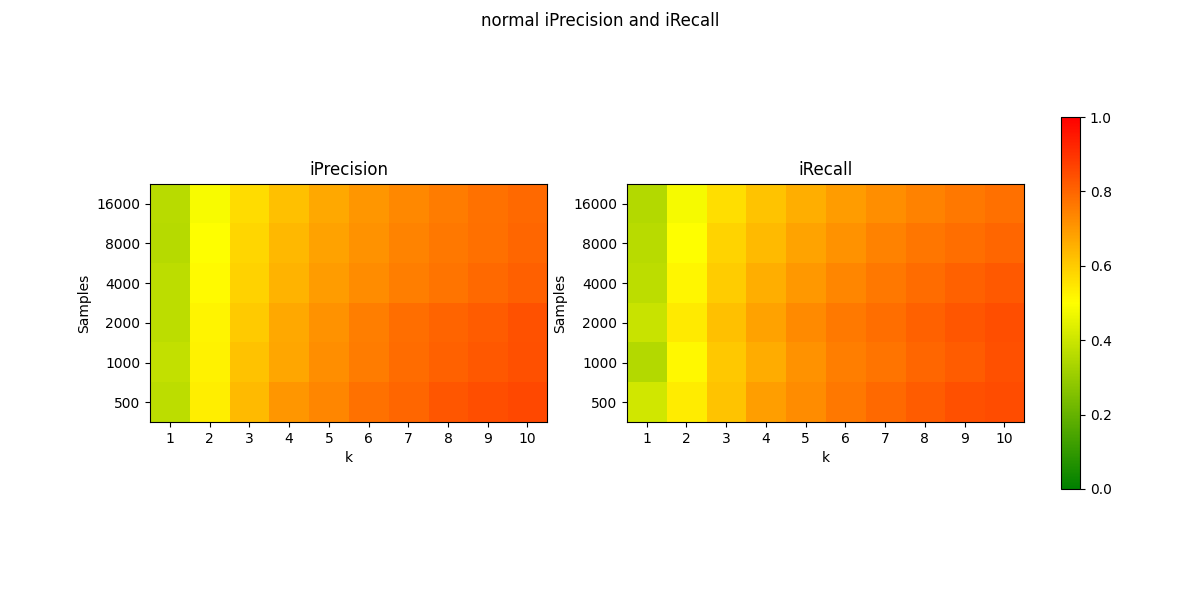
\includegraphics[width=0.8\textwidth]{../images/toyexperiments/kdim/normal_iPrecision_iRecall.png} 
\end{figure}

\begin{figure}[!ht]
    \centering
    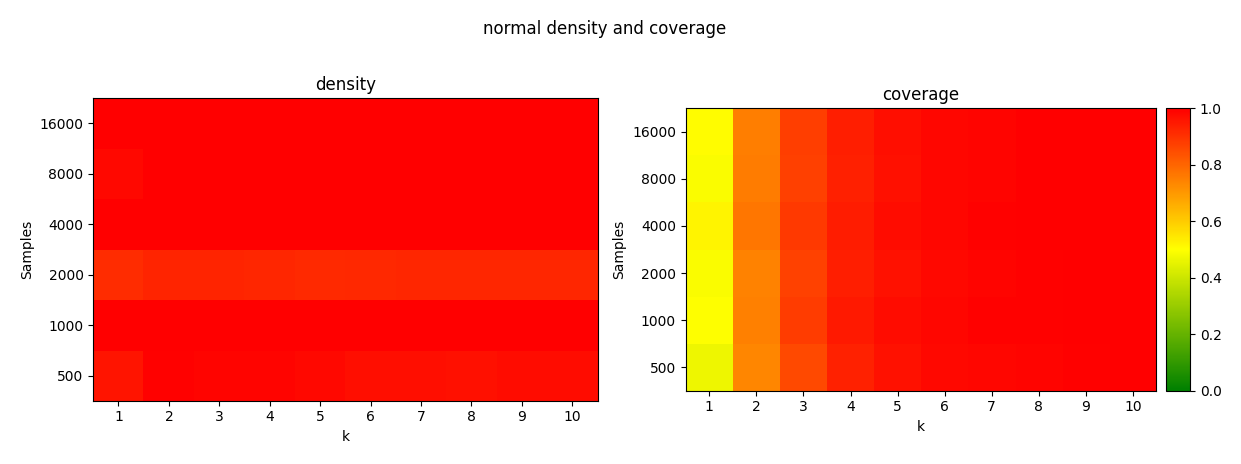
\includegraphics[width=0.8\textwidth]{../images/toyexperiments/kdim/normal_density_coverage.png} 
\end{figure}

Come possiamo notare i risultati ottenuti sono molto simili a quelli presenti nel paper. Essendo le due distribuzioni di dati reali e generati identiche, una metrica che rispecchi tale somiglianza dovrebbe avere valori molto vicini ad \texttt{1.}, in particolar modo quando la dimensione del dataset è molto grande.
Un comportamento simile indicherebbe una buona robustezza della metrica rispetto a variazioni di \texttt{k}, ma come possiamo notare dai grafici, l'improved precision recall è molto più sensibile rispetto ai valori dell'iperparametro. 
Si può notare inoltre una sensibilità maggiore delle metriche al variare di \texttt{k} rispetto alla dimensione del dataset, i grafici sono infatti caratterrizati da colonne verticali di valori/colori molto simili.
La density dall'altra parte è molto più stabile, è però necessario ricordare che per distribuzioni di dati molto simili, non essendo normalizzata, ottenga valori persino maggiori di \texttt{1.}, portando la metrica a non essere molto significativa.
La coverage risulta anch'essa molto stabile, non dando valori molto diversi da \texttt{1.}, ad eccezione per \texttt{k = 1} con dimesione del dataset molto piccola.

Si riportano quindi i risultati per le due metriche ignorate dal paper sempre per distribuzioni normali di dati:

\begin{figure}[!ht]
    \centering
    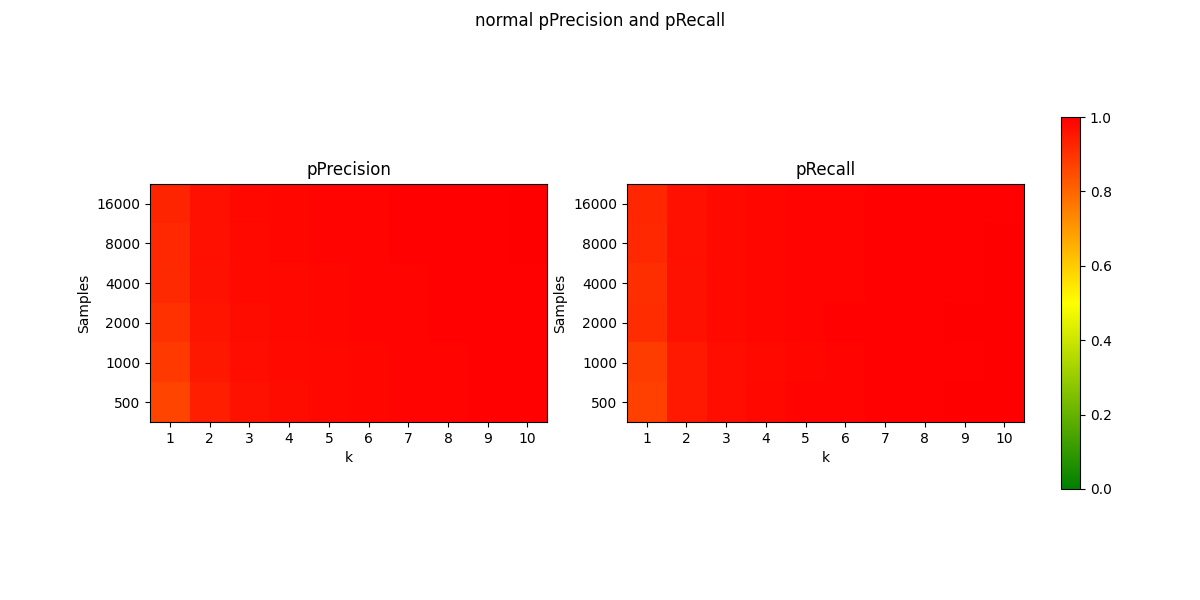
\includegraphics[width=0.8\textwidth]{../images/toyexperiments/kdim/normal_pPrecision_pRecall.png} 
    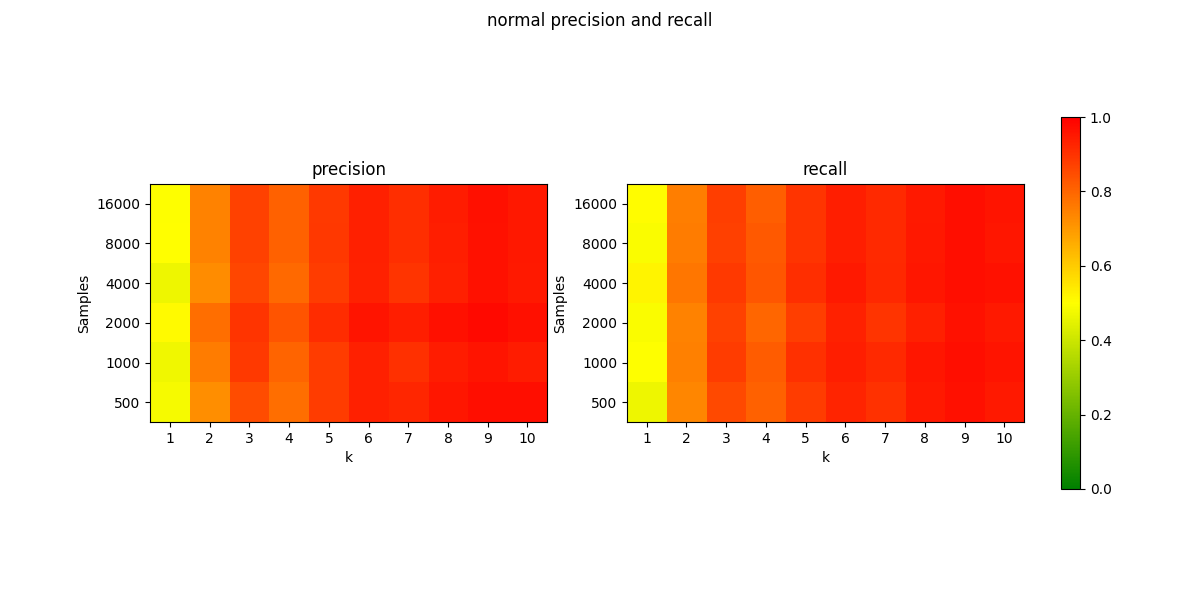
\includegraphics[width=0.8\textwidth]{../images/toyexperiments/kdim/normal_precision_recall.png} 
\end{figure}

In questo caso è apprezzabile l'uniformità di colore nei grafici della probabibilistic precision e recall, indice della corretta stima della sovrapposizione dei supporti dei dataset di eguale distribuzione.
Come per la density però, dobbiamo limitare i ragionamenti induttivi delle capacità della metrica di stimare la somiglianza fra due distribuzioni, a distribuzioni uguali. Questo vuol dire che con distribuzioni diverse la metrica potrebbe non risultare altrettanto sensibile e appunto continuare a dare valori alti quando non dovrebbe,
come si suol dire 'anche un orologio rotto segna l'ora giusta due volte al giorno'. Per la precision-recall coverage invece è interessante notare come per il valore di \texttt{k} consigliato in letteratura (\texttt{k = 3}) questa porti a una stima migliore persino che nel caso di \texttt{k} di valore superiore, dove teoricamente (esclusivamente per distribuzioni identiche), si avrebbe stime migliori. 
Inoltre si può apprezzare la somiglianza fra i grafici della coverage e della precision-coverage, per i quali ricordiamo dalla teoria che con \texttt{k = 1} le due metriche risultano analiticamente identiche.

I risultati degli esperimenti su distribuzioni uniformi identiche sono i seguenti:

\begin{figure}[!ht]
    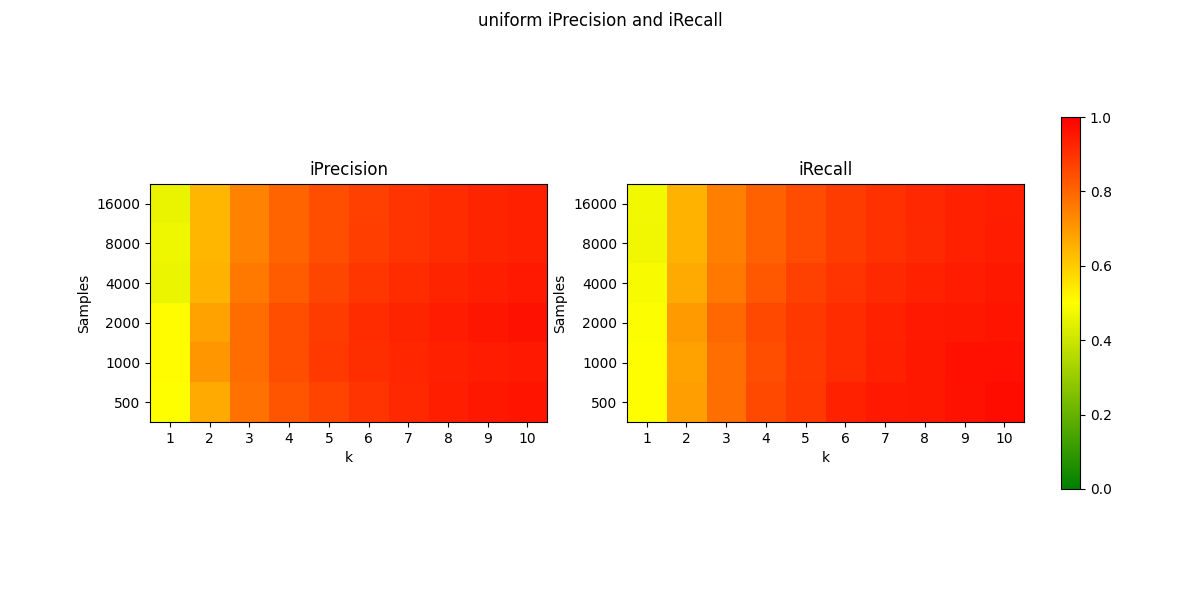
\includegraphics[width=0.5\textwidth]{../images/toyexperiments/kdim/uniform_iPrecision_iRecall.png} 
    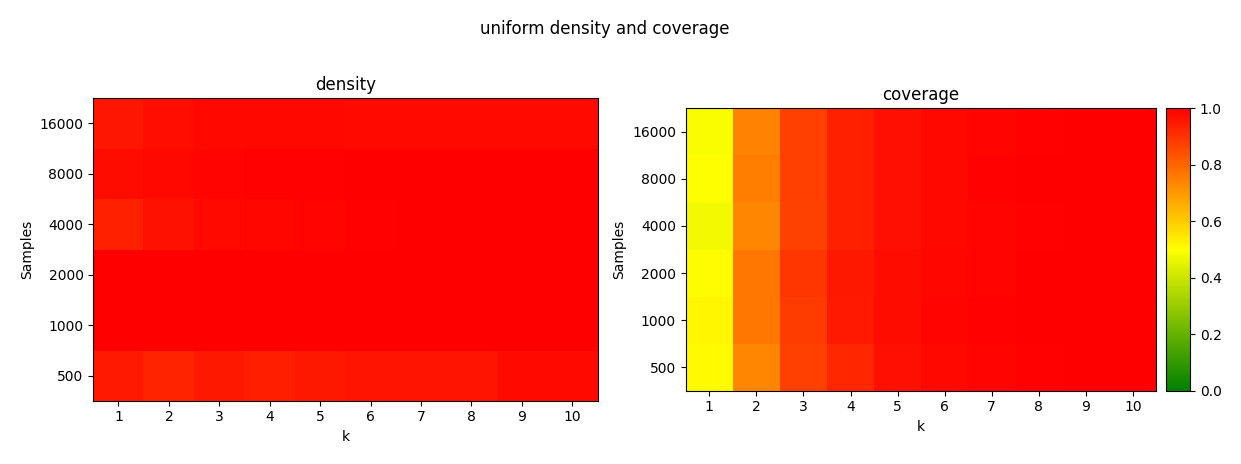
\includegraphics[width=0.5\textwidth]{../images/toyexperiments/kdim/uniform_density_coverage.png} 
    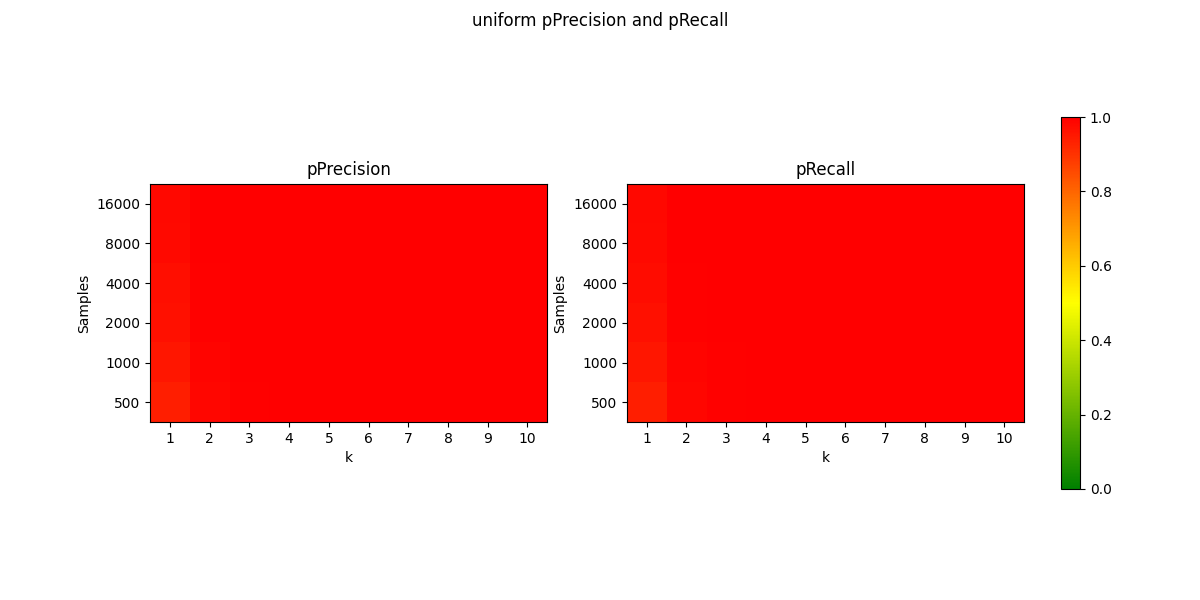
\includegraphics[width=0.5\textwidth]{../images/toyexperiments/kdim/uniform_pPrecision_pRecall.png}
    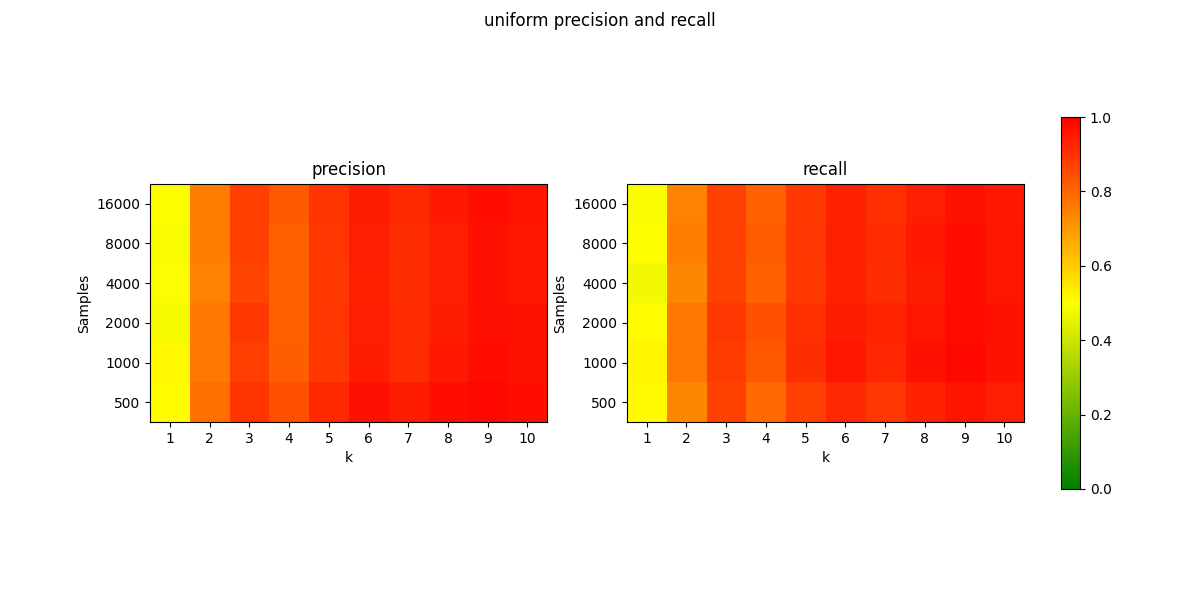
\includegraphics[width=0.5\textwidth]{../images/toyexperiments/kdim/uniform_precision_recall.png} 
\end{figure}

Come risulta a prima vista, non si discostano molto da i grafici ottenuti con distribuzioni normali. Possiamo quindi solo estendere le precedenti conclusioni a questa nuova distribuzione.
Unica eccezione è l'improved precision-recall che presenta risultati migliori in questo caso, segnalando una limitatezza della sensibilità in presenza di \texttt{k} con valori bassi e distribuzioni normali.

\subsection{Dimensione del dataset e dimensione dei dati}

Per quanto riguarda gli esperimenti sulla dimensione dei dati i risultati sono i seguenti:

\begin{figure}[!ht]
    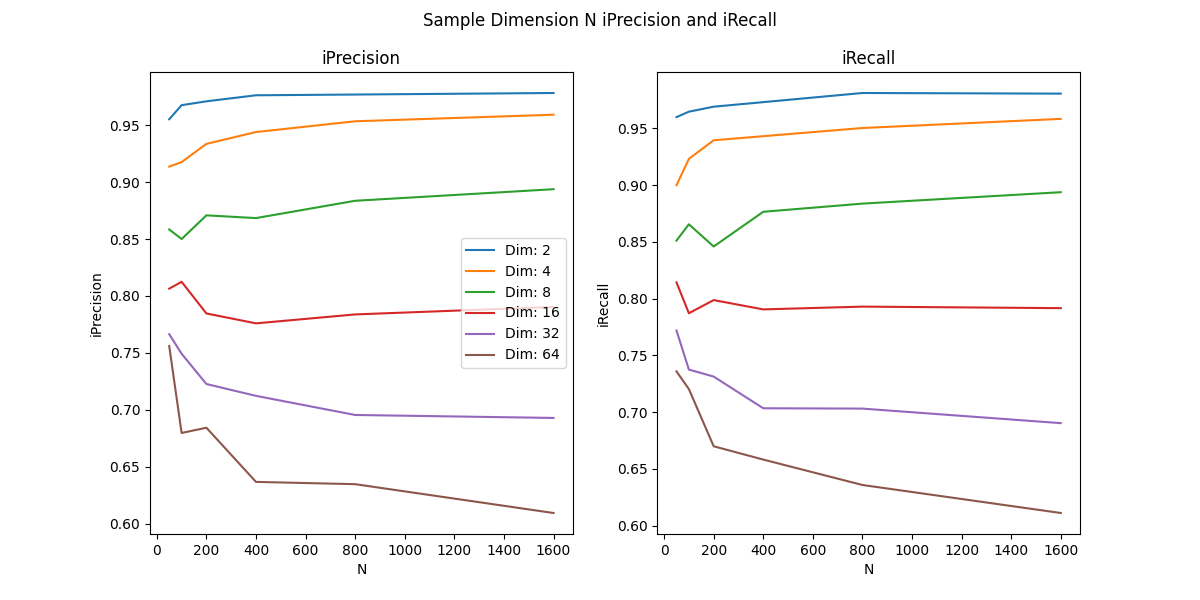
\includegraphics[width=0.5\textwidth]{../images/toyexperiments/ksampledim/sampleDimN_iPrecision_iRecall.png} 
    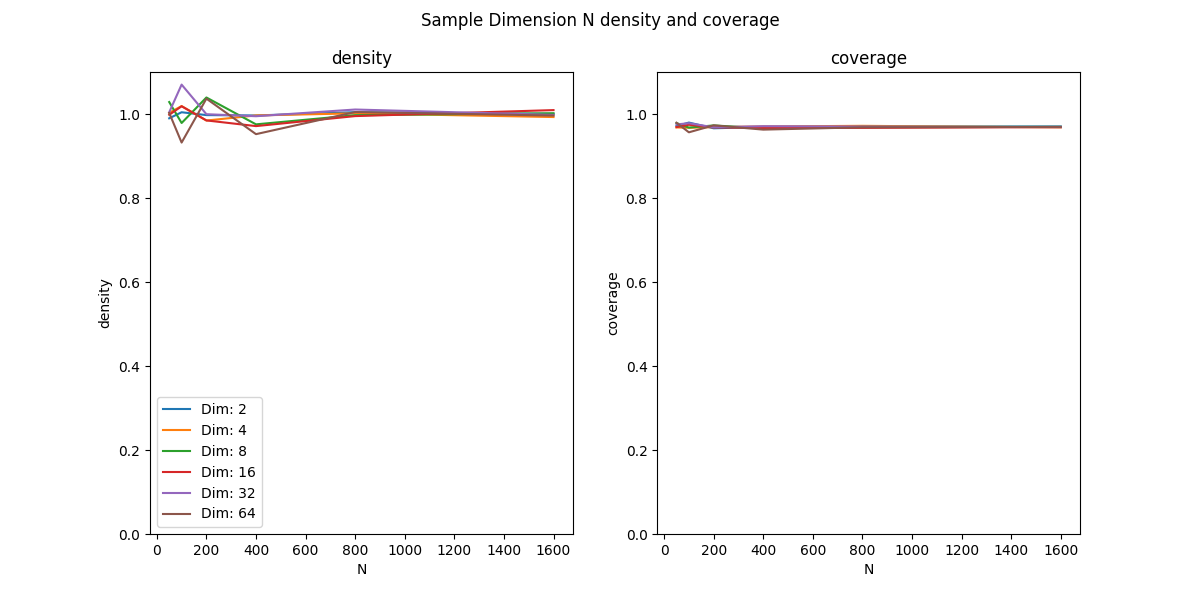
\includegraphics[width=0.5\textwidth]{../images/toyexperiments/ksampledim/sampleDimN_density_coverage.png} 
    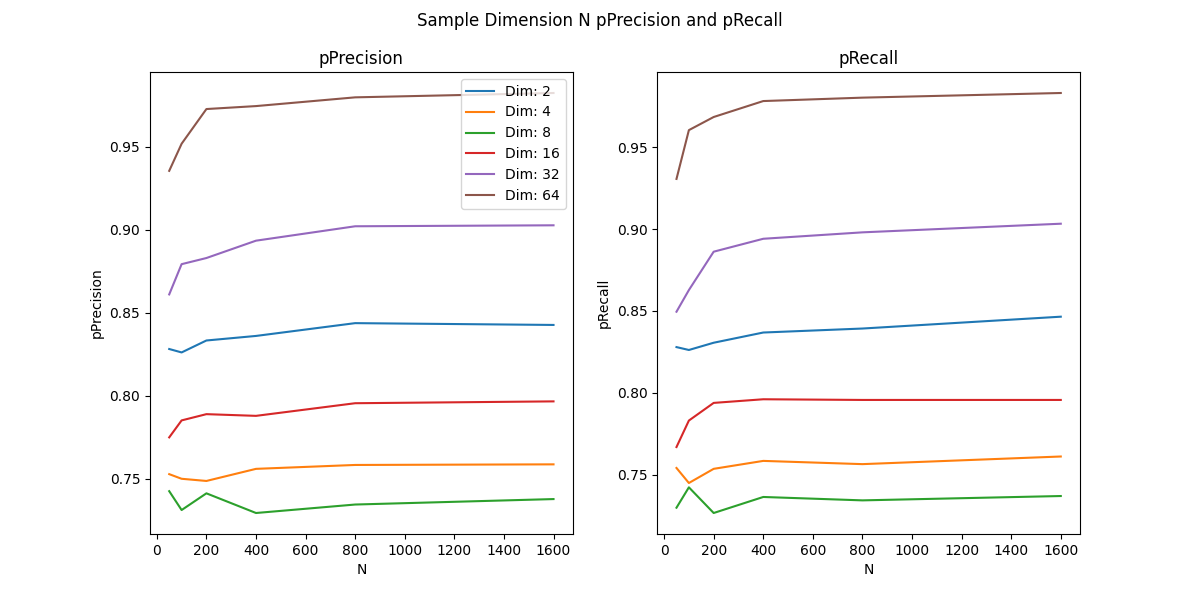
\includegraphics[width=0.5\textwidth]{../images/toyexperiments/ksampledim/sampleDimN_pPrecision_pRecall.png} 
    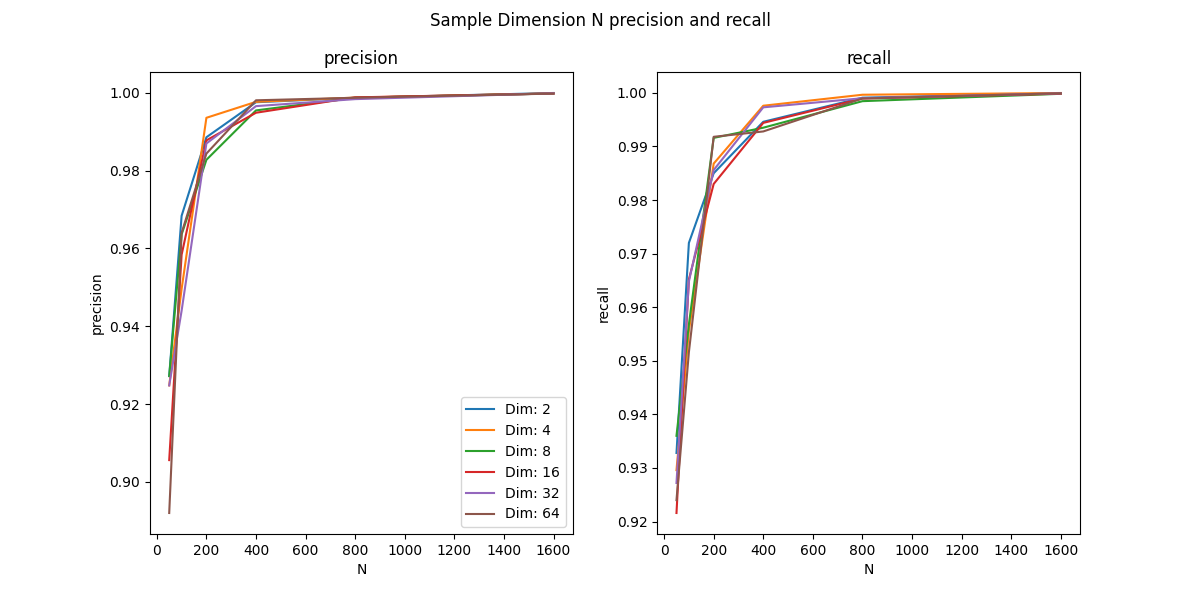
\includegraphics[width=0.5\textwidth]{../images/toyexperiments/ksampledim/sampleDimN_precision_recall.png} 
\end{figure}

Le uniche due metriche che risultano sensibili alla variazione della dimensione dei dati sono la improved precision-recall e la probabibilistic precision-recall, mentre le altre due risultano molto stabili.
L'asse delle ascisse è stata limitata leggermente sopra a \texttt{1.} (\texttt{1.25}) possiamo quindi apprezzare visimamente una delle proprietà di cui abbiamo accennato nella sezione precedente e nel primo capitolo:
la density non essendo normalizzata presenta valori che superano il limite logico delle condiviso dalle altre metriche.

Per l'improved precision recall si individua la fragilità della metrica alla dimensione dei dati. Per dimensioni elevate, a parità di numero di campioni e di distribuzione, si registra valori di precision e recall inferiori.
Risulta infatti che per dati in \(\mathbb{R}^{64}\) i valori della metrica siano inferiori di circa 30 punti percentuale rispetto a i dati in  \(\mathbb{R}^{2}\).

Per la probabilistic precision recall è sempre presente questa fragilità, ma non è ben chiaro come la dimensione dei dati sia legata agli effettivi risultai della metrica, risulta infatti che per le due dimensioni dei dati maggiori
testate i valori della metrica siano migliori ma con essi è presente anche la dimensione dei dati minore testata, mentre per \(\mathbb{R}^{8}\) otteniamo la stima più bassa.

\subsection{Outliers}

I casi di studio, come detto nel capitolo precedente sono tre: valori della metrica per distribuzioni normali di dati reali e generate, con la distribuzione dei dati generati centrata nei diversi valori dell'ordinata senza outliers, con outliers nei dati reali e con outliers nei dati generati.

I risultati ottenuti per l'improved precision-recall sono i seguenti:

%need to go to the next page
\clearpage

\begin{figure}[!ht]
    \centering
    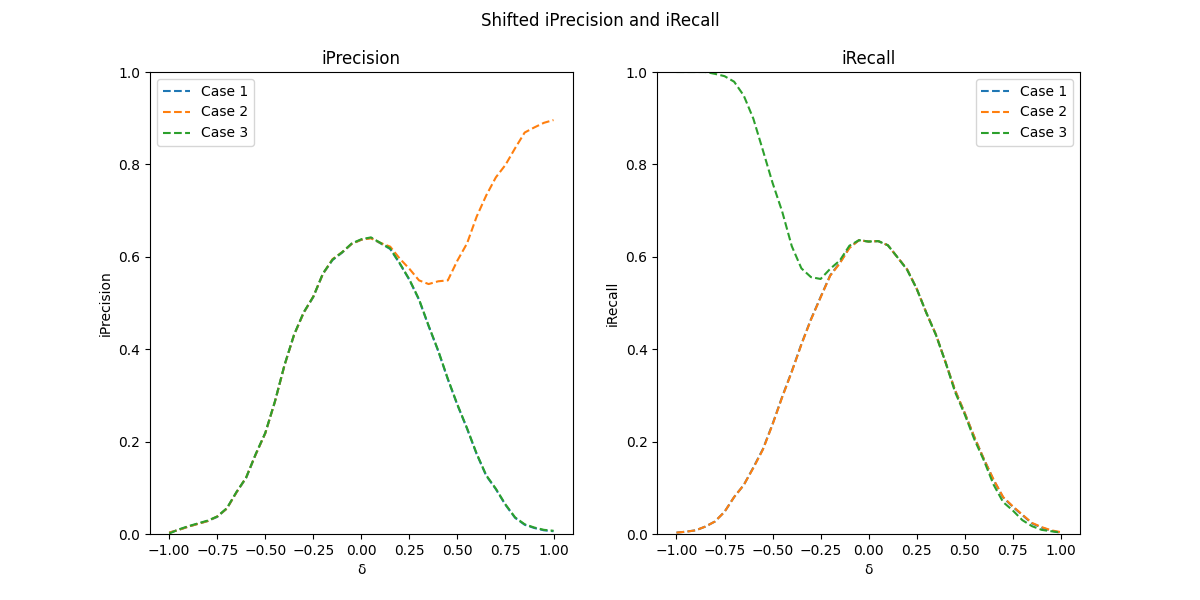
\includegraphics[width=0.8\textwidth]{../images/toyexperiments/outliers/shift_iPrecision_iRecall.png} 
\end{figure}

È possibile notare che i risultati ottenuti rispettano quanto atteso dalla letteratura. La metrica risulta essere molto sensibile alla presenza di outliers nei dati.
In particolare la precision risulta essere estremamente sensibile alla presenza di outliers nei dati reali, poichè questi vanno a determinare una sovrastimare dell'area del manifold di \(R\), dall'altra parte 
la recall risulta essere molto sensibile alla presenza di outliers nei dati generati, poichè in questo caso si va a sovrastimare l'area del manifold di \(G\).
Un singolo dato outlier può far variare la metrica dell'80\% rispetto al caso senza outliers.
Un altro problema grave delle due metriche è che quando lo shift fra le due distribuzioni è \texttt{0.} la metrica è molto più bassa di \texttt{1.}, paradossalmente viene registrato un valore maggiore dei manifold per distribuzioni con media spostata rispetto a distribuzioni con media centrata.

I risultati ottenuti per la density-coverage sono i seguenti:

\begin{figure}[!ht]
    \centering
    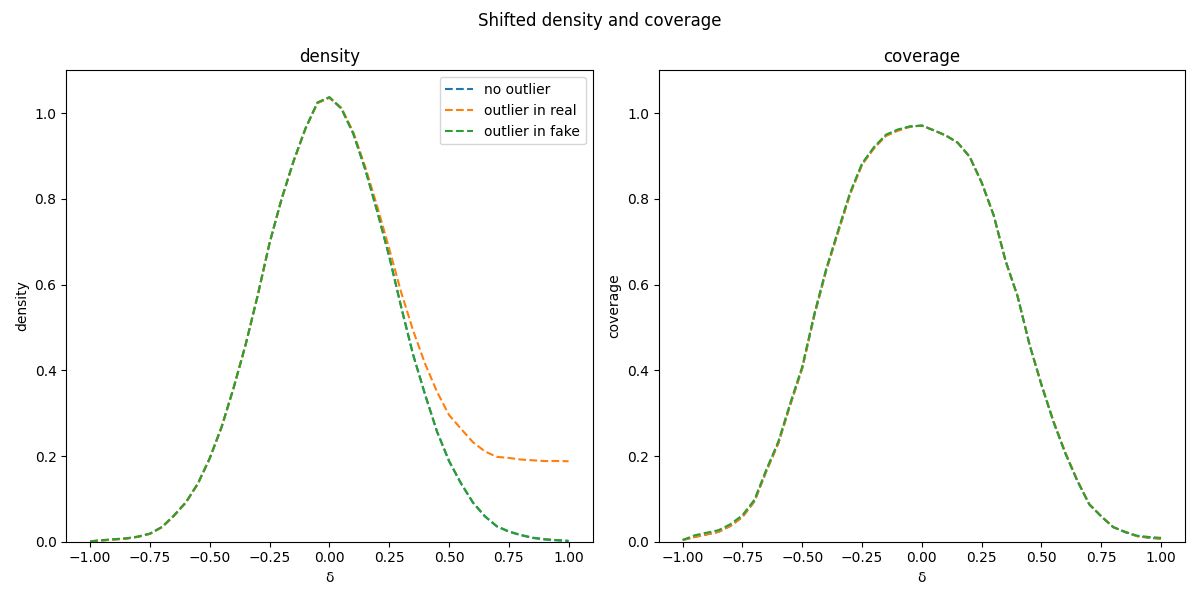
\includegraphics[width=0.8\textwidth]{../images/toyexperiments/outliers/shift_density_coverage.png} 
\end{figure}

Ancora una volta i risultati ottenuti rispettano quanto atteso dalla letteratura. La metrica risulta essere molto robusta alla presenza di outliers nei dati.
La density è leggermente influenzata dalla presenza di outliers nei dati reali, ma non in maniera significativa, mentre la coverage non risente della presenza di outliers sia nei dati reali che nei dati generati.
Al contrario dell'improved precision recall, la density e la coverage hanno valori molto vicini a \texttt{1.} quando lo shift fra le due distribuzioni è \texttt{0.} (la density non essendo normalizzata ha valori maggiori di \texttt{1.}).

Per le altre due metriche non indagate nel paper i risultati sono i seguenti:

\begin{figure}[!ht]
    \centering
    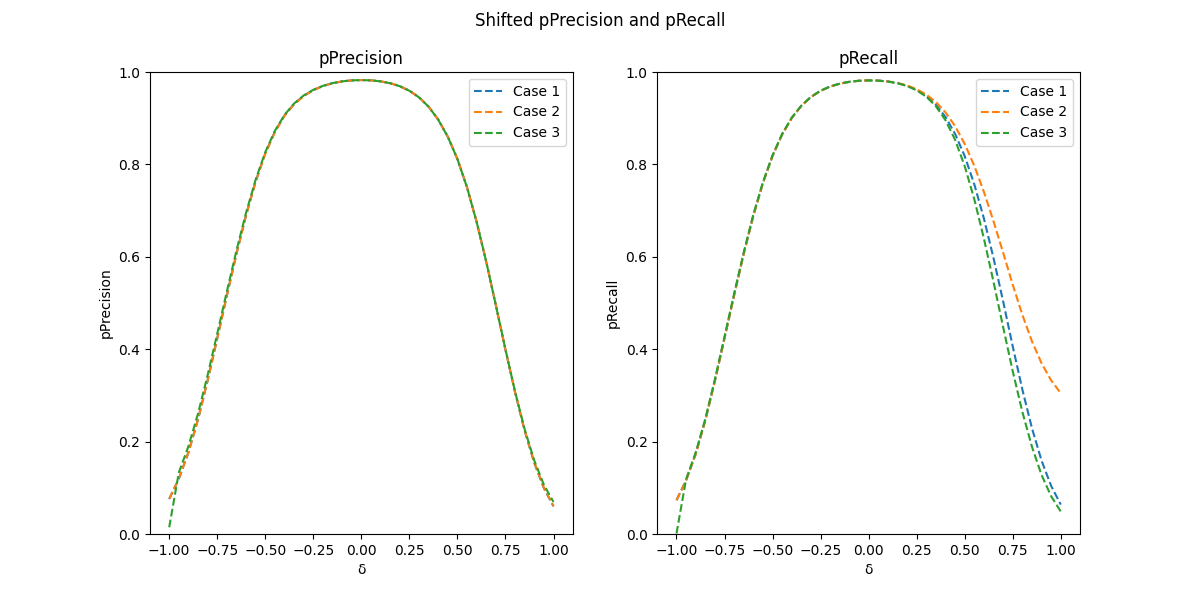
\includegraphics[width=0.8\textwidth]{../images/toyexperiments/outliers/shift_pPrecision_pRecall.png} 
    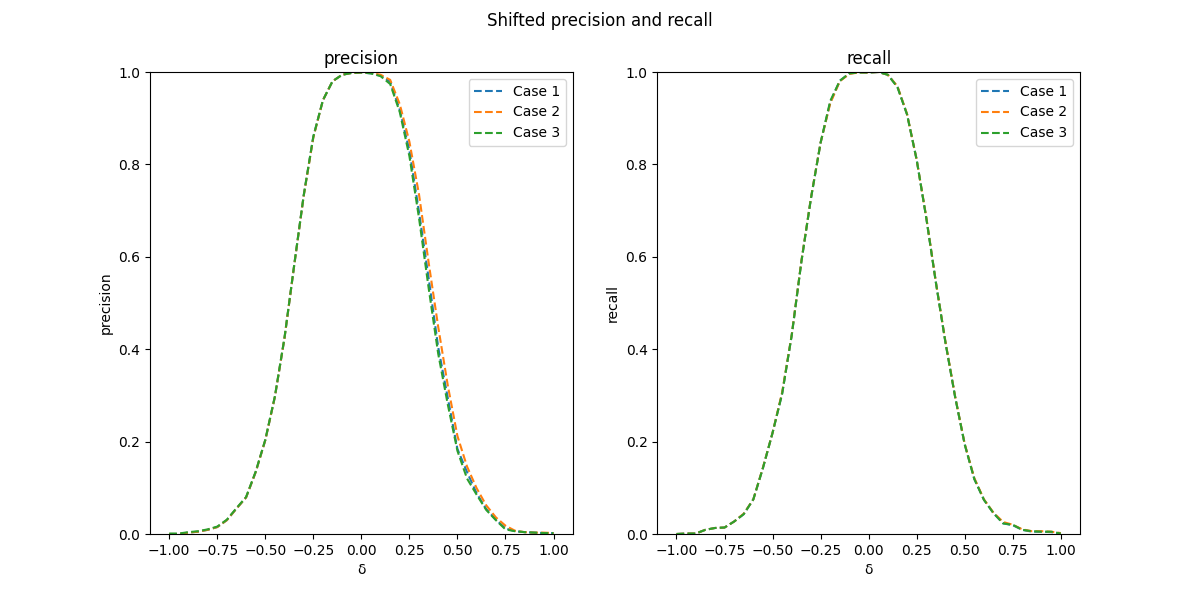
\includegraphics[width=0.8\textwidth]{../images/toyexperiments/outliers/shift_precision_recall.png} 
\end{figure}

Come per la density e coverage, le due metriche più recenti risultano essere molto robuste alla presenza di outliers nei dati e misurano correttamente la sovrapposizione dei manifold delle due distribuzioni in assenza di shift.
Data la diversa natura delle due metriche, la probabibilistic precision-recall presenta valori più alti lo shift è non nullo.

\subsection{Comparazione con implementazioni esistenti e riproduzione delle pr-curves}

Come avevamo anticipato nell'introduzione dei ToyData experiments, abbiamo verificato che le implementazioni linkate nei vari paper presi in esame riportassero risultati conformi a quelli ottenuti con la nostra implementazione.
Per fare ciò, oltre a riprodurre esperimenti simili a quelli presenti nei paper e confrontato i grafici come visto sino ad adesso, abbiamo verificato numericamente che i valori delle metriche fossero effettivamente gli stessi.
Una rapida presa visione del codice sorgente ha permesso di verificare delle differenze implementative che però sono risultate indifferenti se non in termini di complessità computazionale.

Per quanto riguarda le implementazioni di improved precision-recall \cite{2ImprovedPrecisionRecall} i risultati ottenuti sono identici per tutte e tre le distribuzioni di dati presi in analisi.

Per le implementazioni di improved precision-recall e density-coverage \cite{3ReliableFidelityDiversityMetrics} i risultati ottenuti sono identici per tutte e tre le distribuzioni di dati presi in analisi.

Per le implementazioni di probabilistic precision-recall \cite{4ProbabilisticPrecisionRecall} i risultati ottenuti differiscono alla 15esima cifra significativa per tutte e tre le distribuzioni di dati presi in analisi.
Tale differenza non è significativa e può essere attribuita a errori numerici dovuti alla precisione di calcolo delle macchine. Per il calcolo della probabibilistic precision-recall è necessario anche il calcolo della \(\rho(\Phi)\) che è come visto nel capitolo 1 una media delle \texttt{k}-NN distances,
e nei nostri esperimenti risulta che anche la misura di questa distanza risulta essere equivalente a quella calcolata dalle implementazioni dei papers.

Passiamo ora alla comparazione delle pr-curves. In questo caso le pr-curves riprodotte dipendevano dalla scelta del parametro \texttt{k}, dallo shift fra le due distribuzioni e dallo split del traing set e del test set.
Per i dataset normali con split del 50\% abbiamo ottenuto i seguenti risultati:

\begin{figure}[!ht]
    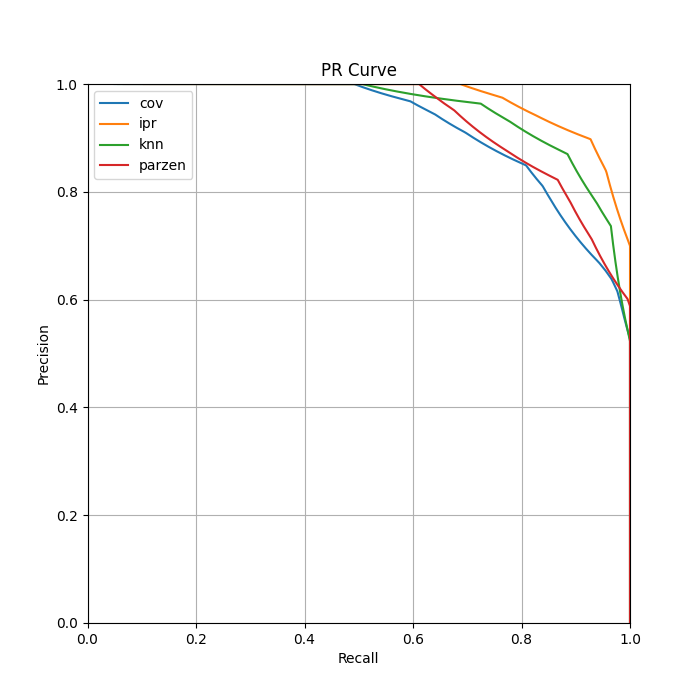
\includegraphics[width=0.5\textwidth]{../images/toyexperiments/prcurves/PRCurve_k4_s1.png} 
    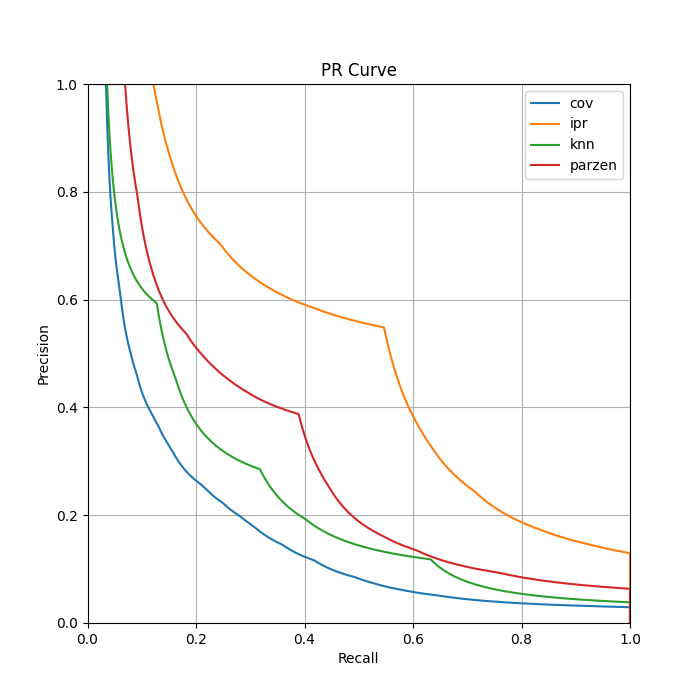
\includegraphics[width=0.5\textwidth]{../images/toyexperiments/prcurves/PRCurve_k4_s3.png}
    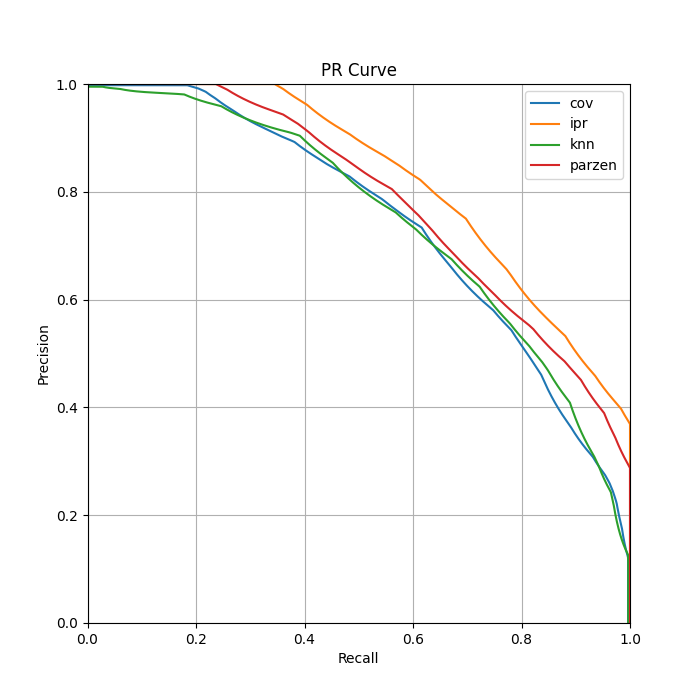
\includegraphics[width=0.5\textwidth]{../images/toyexperiments/prcurves/PRCurve_ksqrt_s1.png} 
    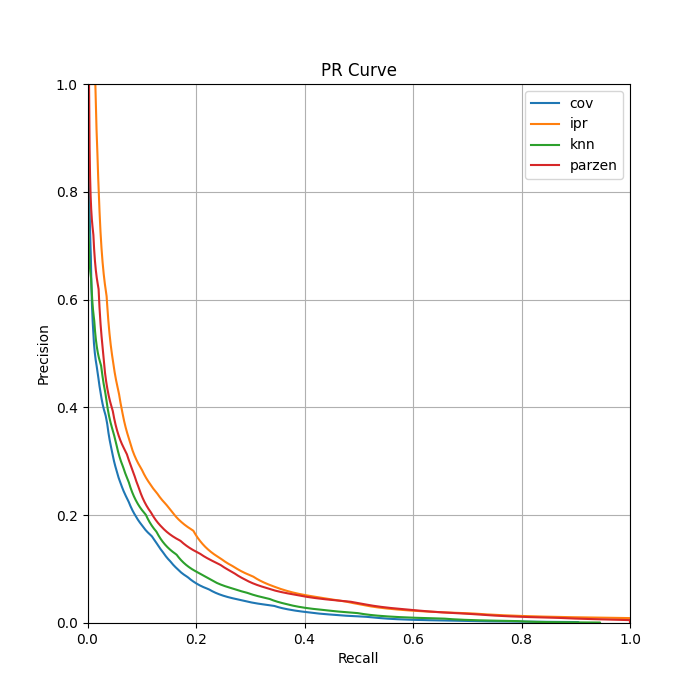
\includegraphics[width=0.5\textwidth]{../images/toyexperiments/prcurves/PRCurve_ksqrt_s3.png} 
\end{figure}


Per i dataset normali senza split abbiamo ottenuto i seguenti risultati:

\begin{figure}[!ht]
    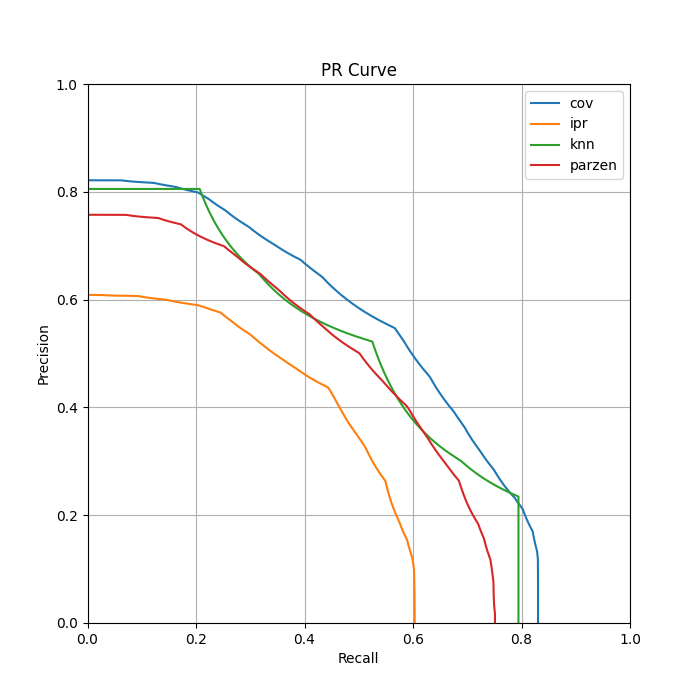
\includegraphics[width=0.5\textwidth]{../images/toyexperiments/prcurves/PRCurve_nosplit_k4_s1.png}
    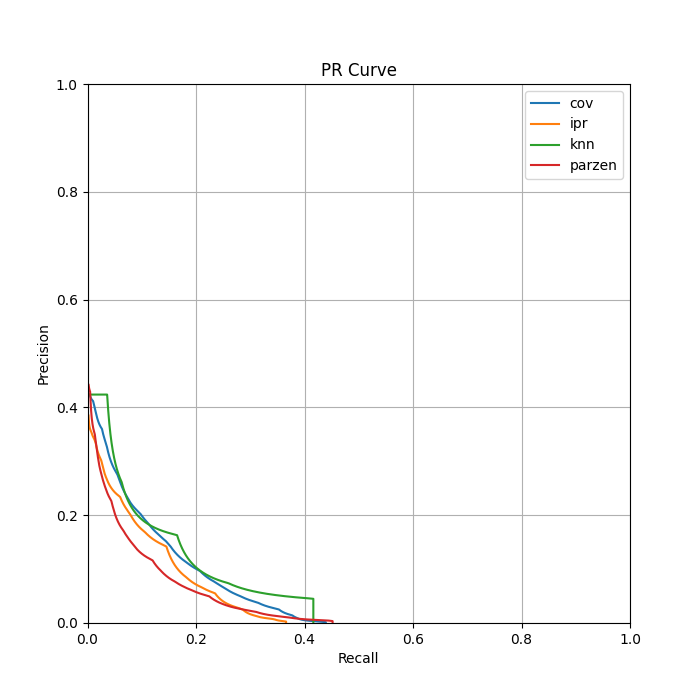
\includegraphics[width=0.5\textwidth]{../images/toyexperiments/prcurves/PRCurve_nosplit_k4_s3.png}
    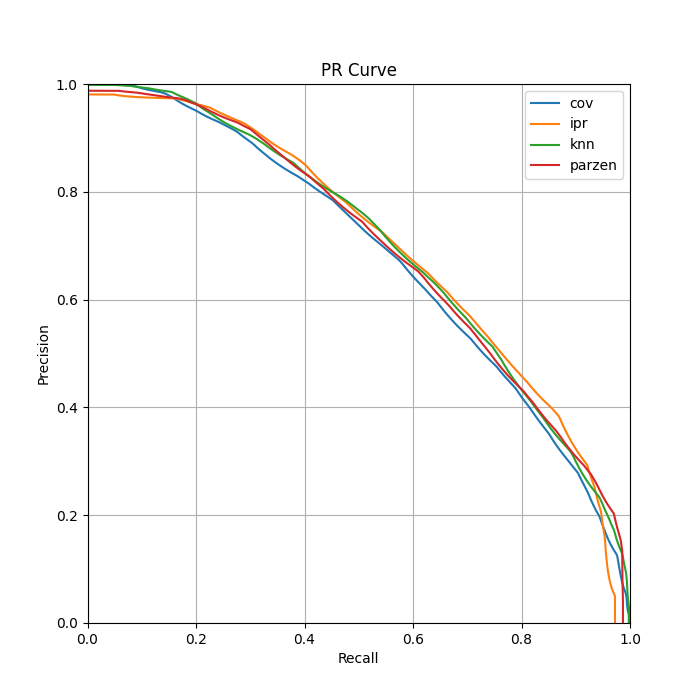
\includegraphics[width=0.5\textwidth]{../images/toyexperiments/prcurves/PRCurve_nosplit_ksqrt_s1.png}
    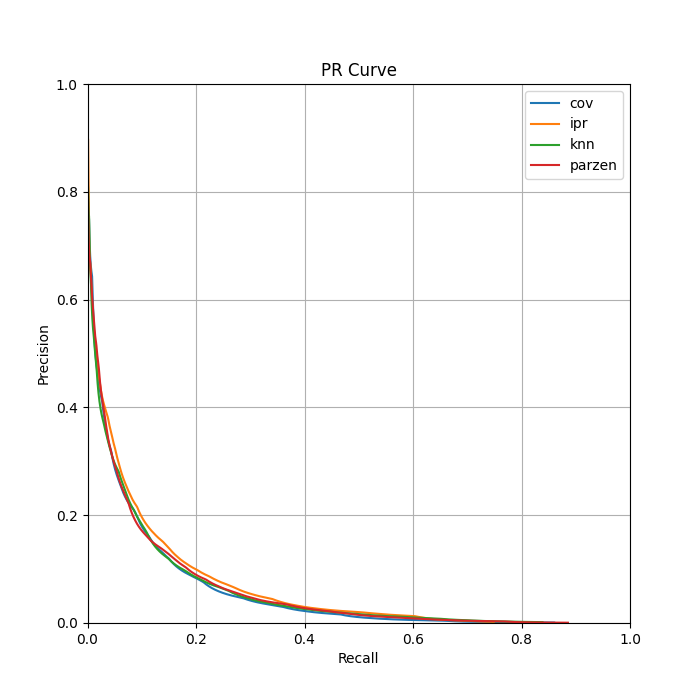
\includegraphics[width=0.5\textwidth]{../images/toyexperiments/prcurves/PRCurve_nosplit_ksqrt_s3.png}
\end{figure}

Anche in questo caso i risultati ottenuti sono conformi a quelli attesi e presenti nei paper. Le conclusioni che si possono trarre sono pertanto le stesse di quelle presenti nei paper, vale a dire che si nota una maggiore stabilità delle pr-curves in presenza di uno split del dataset e con \texttt{k = \(\sqrt{|\Phi|}\)}.

\section{Risultati degli esperimenti su dataset reali}

\subsection{Butterflies}

Prima di condurre gli esperimenti per identificare se le metriche possano operare correttamente da filtro per la selezione di dati generati di alta qualità, abbiamo condotto degli esperimenti preliminari per studiare il dominio in cui avrebbero operato le metriche.
In particolare abbiamo analizzato le kde delle divese caratterristiche proposte per le distanze inter e intra set. L'obbiettivo era quello di verificare che tali caratterristiche fossero sufficientemente descrittive per poter distinguere dati generati di alta qualità da dati generati di bassa qualità.
I risultati ottenuti sono i seguenti:

\begin{figure}[!ht]
    \centering
    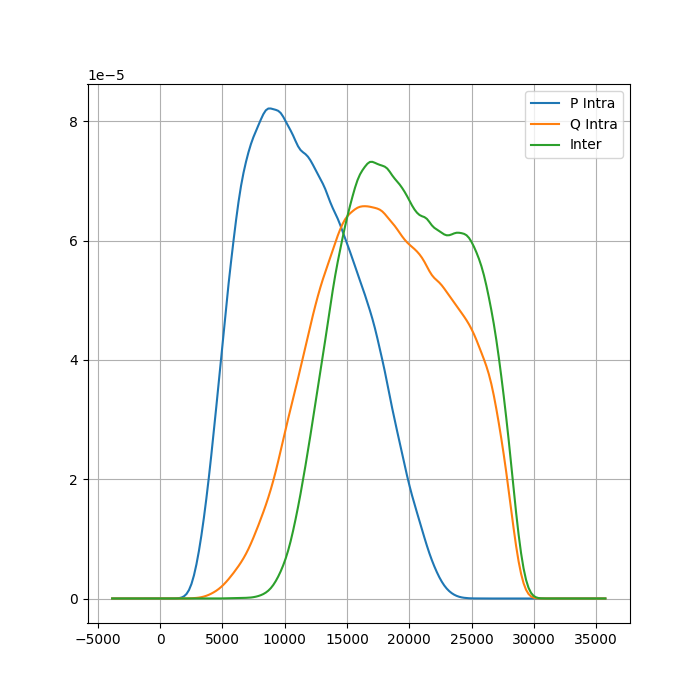
\includegraphics[width=0.3\textwidth]{../images/realworldexperiments/butterflies/kde/kde_grayscale_histogram.png}
    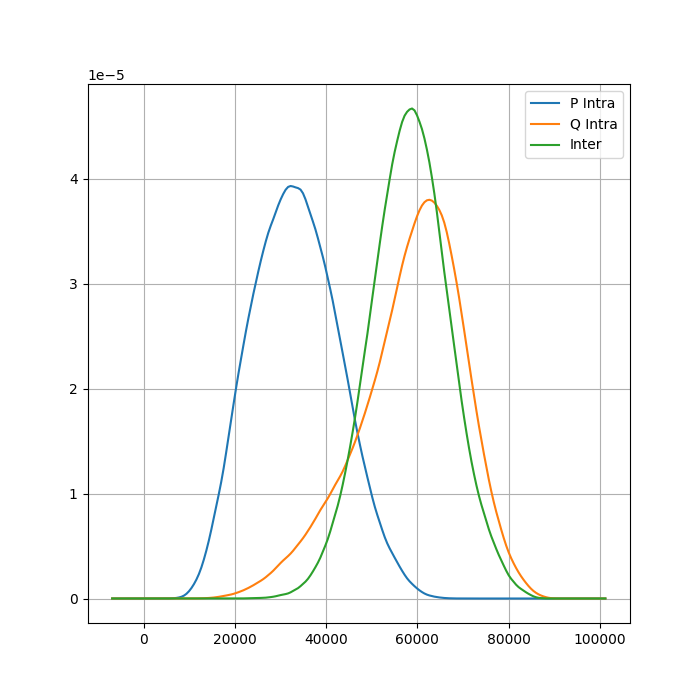
\includegraphics[width=0.3\textwidth]{../images/realworldexperiments/butterflies/kde/kde_hsv_histogram.png}
    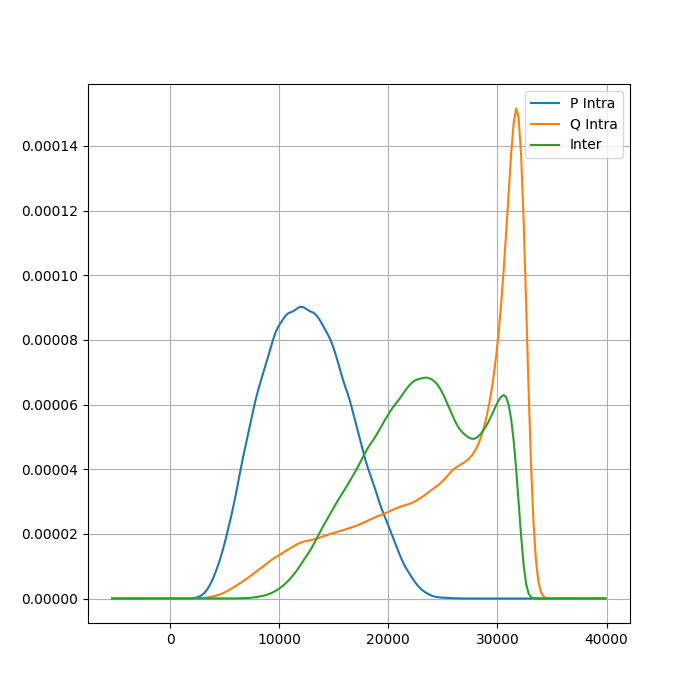
\includegraphics[width=0.3\textwidth]{../images/realworldexperiments/butterflies/kde/kde_hue_histogram.png}
\end{figure}
\begin{figure}[!ht]
    \centering
    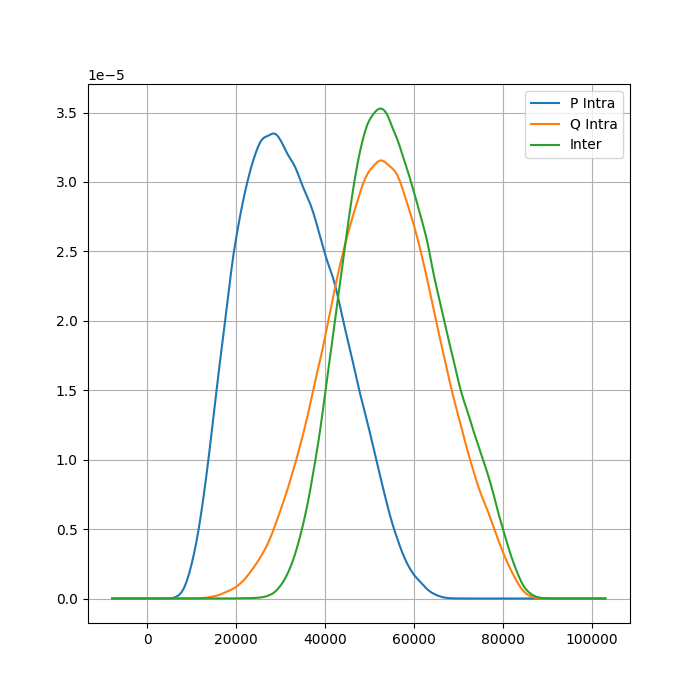
\includegraphics[width=0.3\textwidth]{../images/realworldexperiments/butterflies/kde/kde_rgb_histogram.png}
    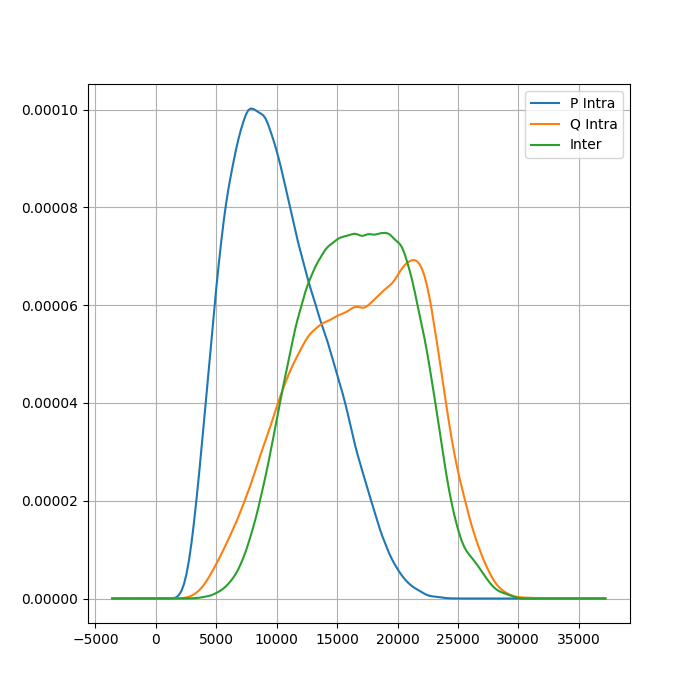
\includegraphics[width=0.3\textwidth]{../images/realworldexperiments/butterflies/kde/kde_saturation_histogram.png}
    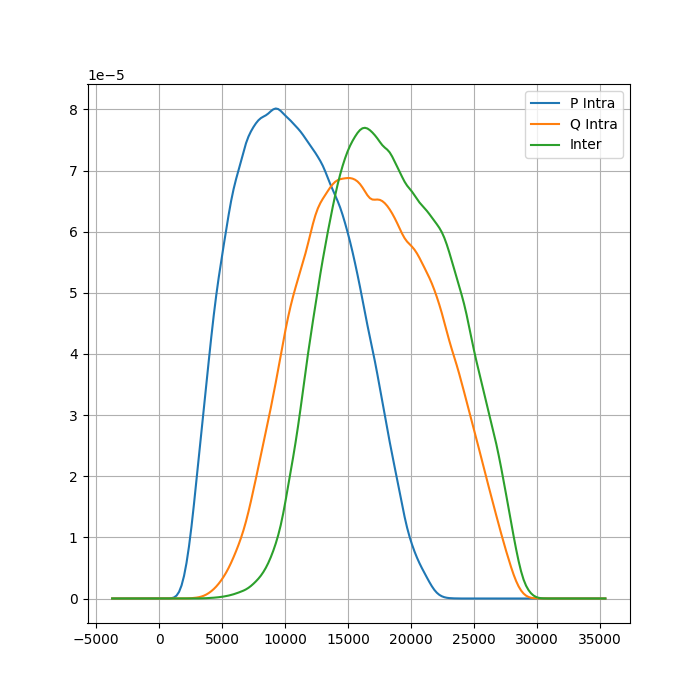
\includegraphics[width=0.3\textwidth]{../images/realworldexperiments/butterflies/kde/kde_value_histogram.png}
    \caption{l'ordine delle immagini da sinistra a destra e dall'alto in basso è: grayscale, hsv, hue, rgb, saturation, value}
\end{figure}

Come si può notare rapidamente per nessuna delle caratterristiche proposte si ha una buona sovrapposizione fra i dati reali e i dati generati. Questo è un segnale che le metriche proposte potrebbero non essere sufficientemente descrittive per poter distinguere i dati generati di alta qualità da quelli generati di bassa qualità,
di fatto un dato generato che risulti outlier per una delle kde calcolate potrebbe comunque essere un dato di alta qualità. Questo è un problema che si ripercuoterà anche nei risultati degli esperimenti successivi.
Come era chiaro fin dall'inizio, un'estrattore che si basa esclusivamente sulle caratteristiche cromatiche e non spaziali non è sufficientemente potente.
L'unica caratteristica in cui abbiamo una sostanziale sovrapposizione fra i dati reali e i dati generati è la value.

A questo punto sono state identificati degli esemplari di falsi positivi con rispettive immagini reali più simili e veri positivi. I risultati ottenuti sono i seguenti:
La selezione si è basata interamente su quei dati che ricadevano o meno nel manifold definito dall'improved precision recall, che come visto dagli esperimenti sui toy dataset soffre della presenza di outliers.
I risultati ottenuti sono i seguenti:

\begin{figure}[!ht]
    \centering
    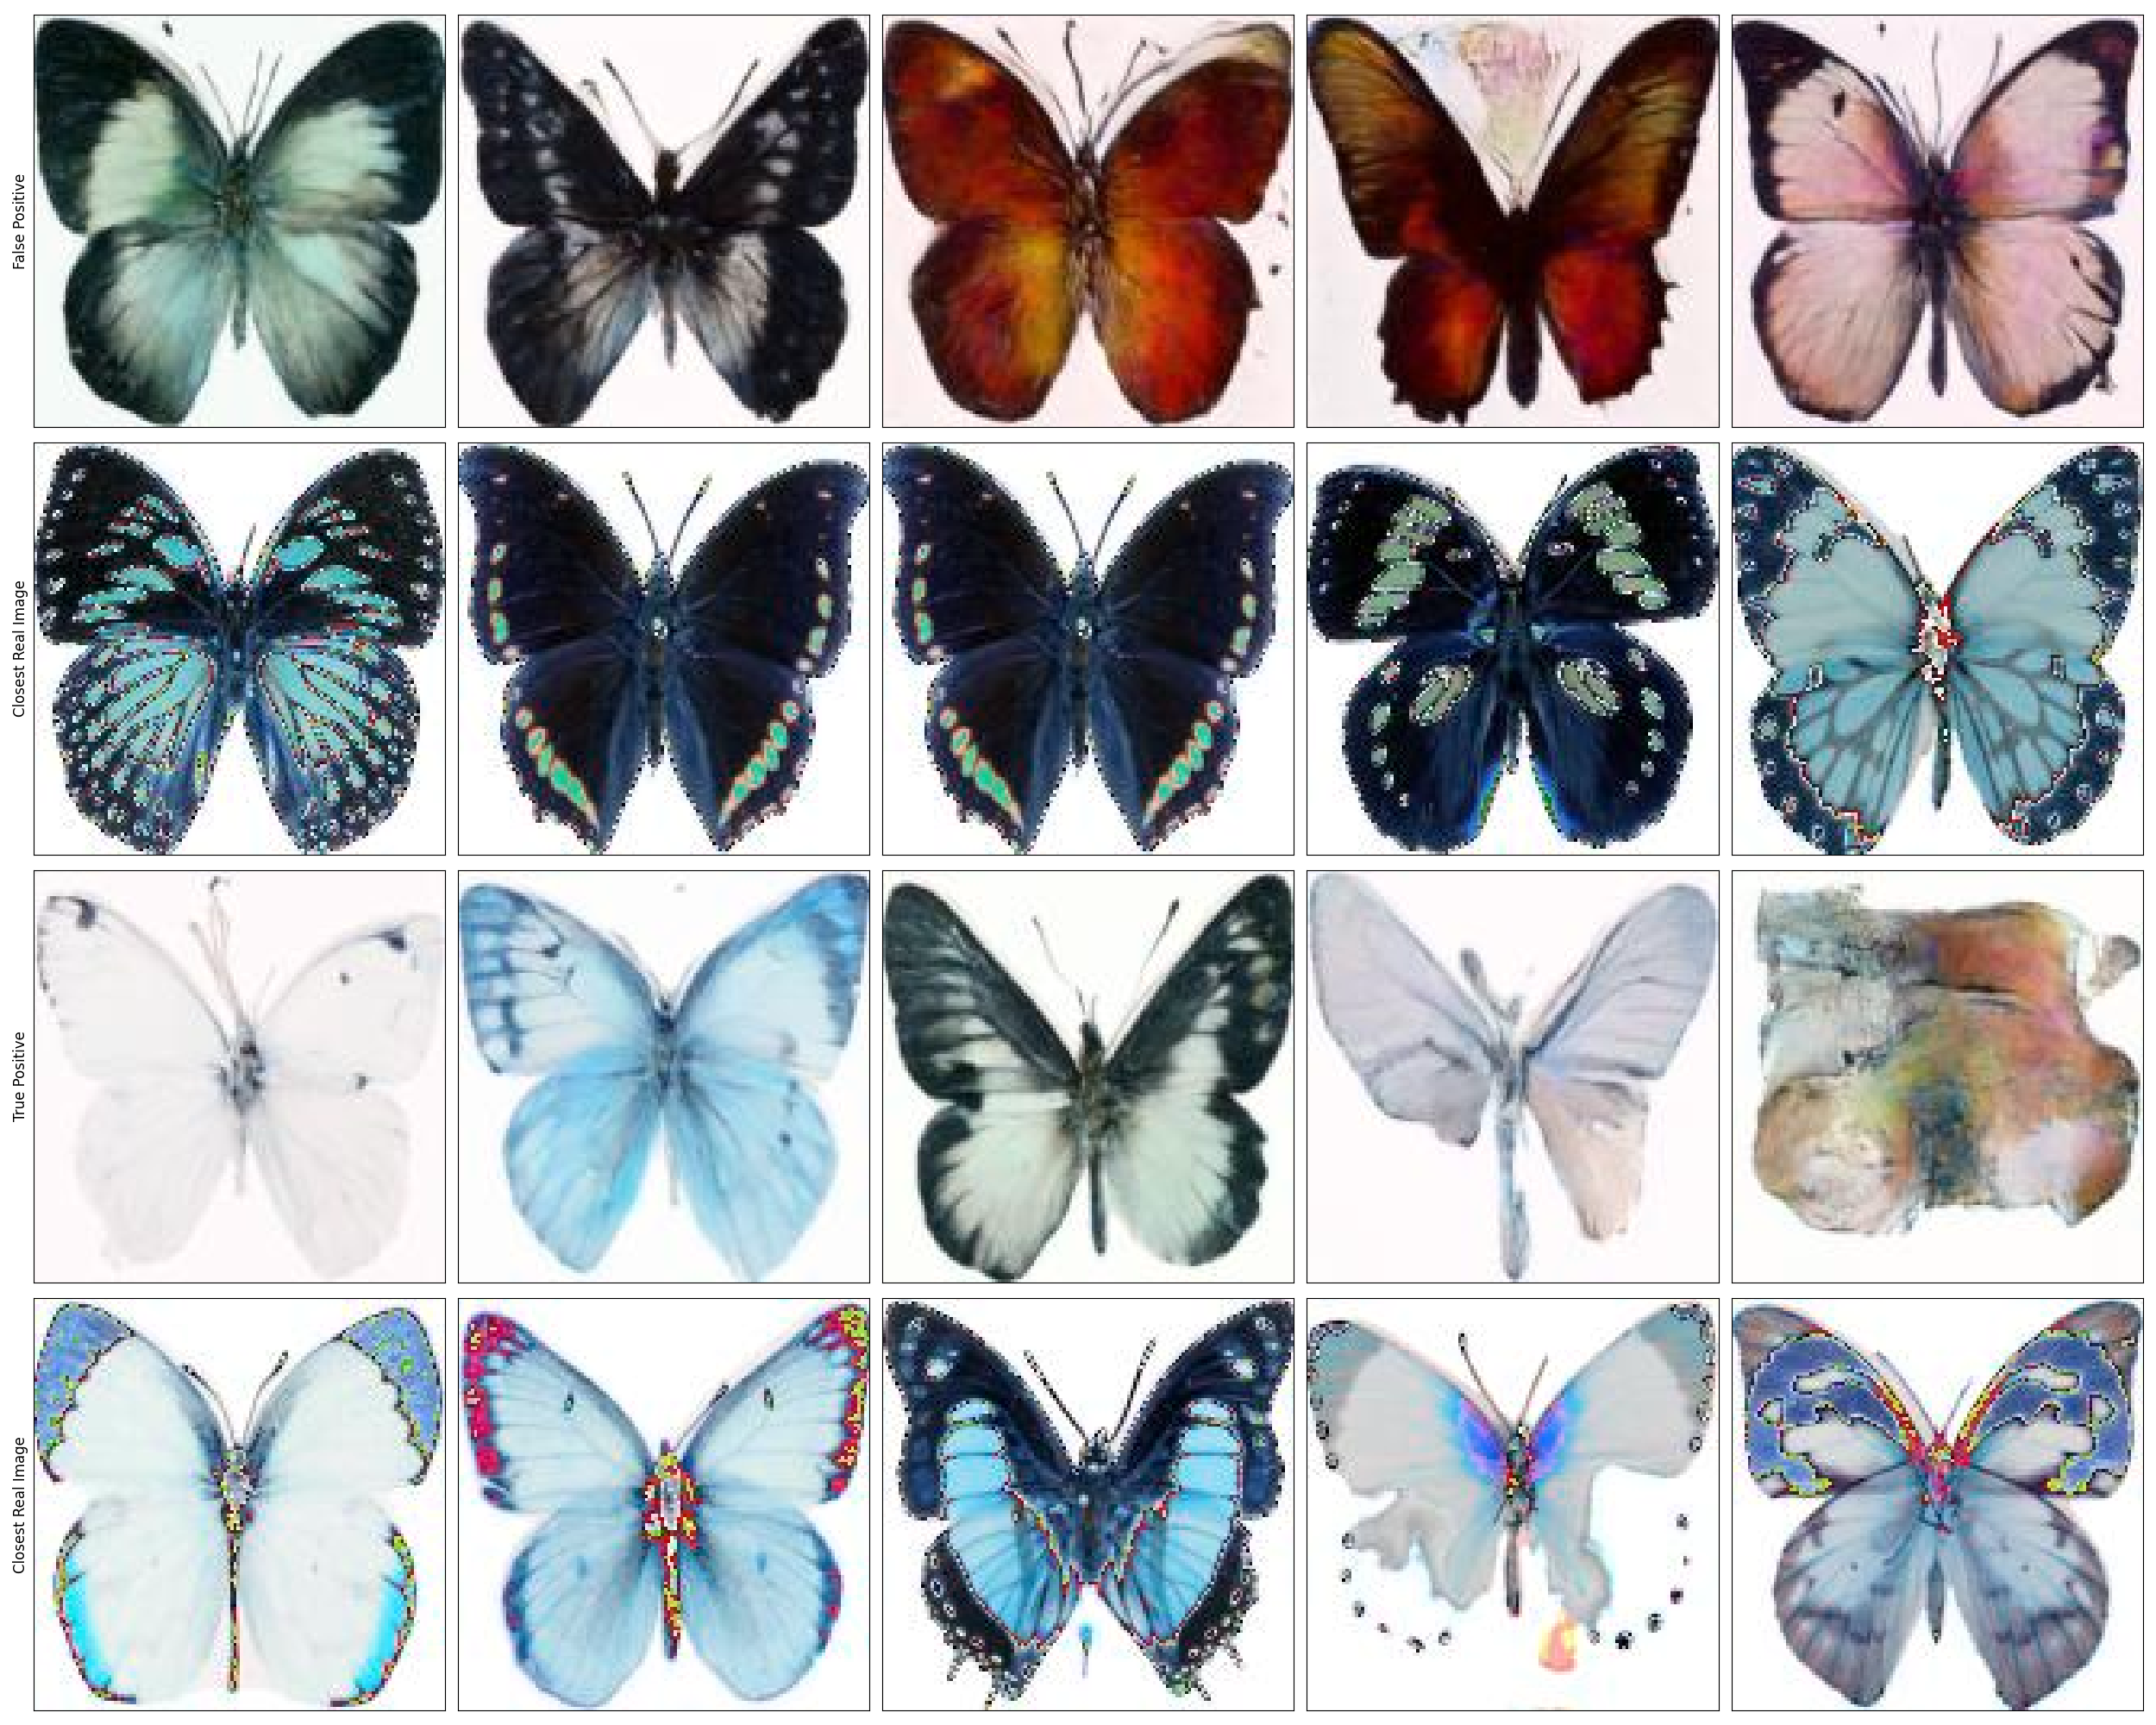
\includegraphics[width=0.45\textwidth]{../images/realworldexperiments/butterflies/examples/fp_grayscale_histogram.png}
    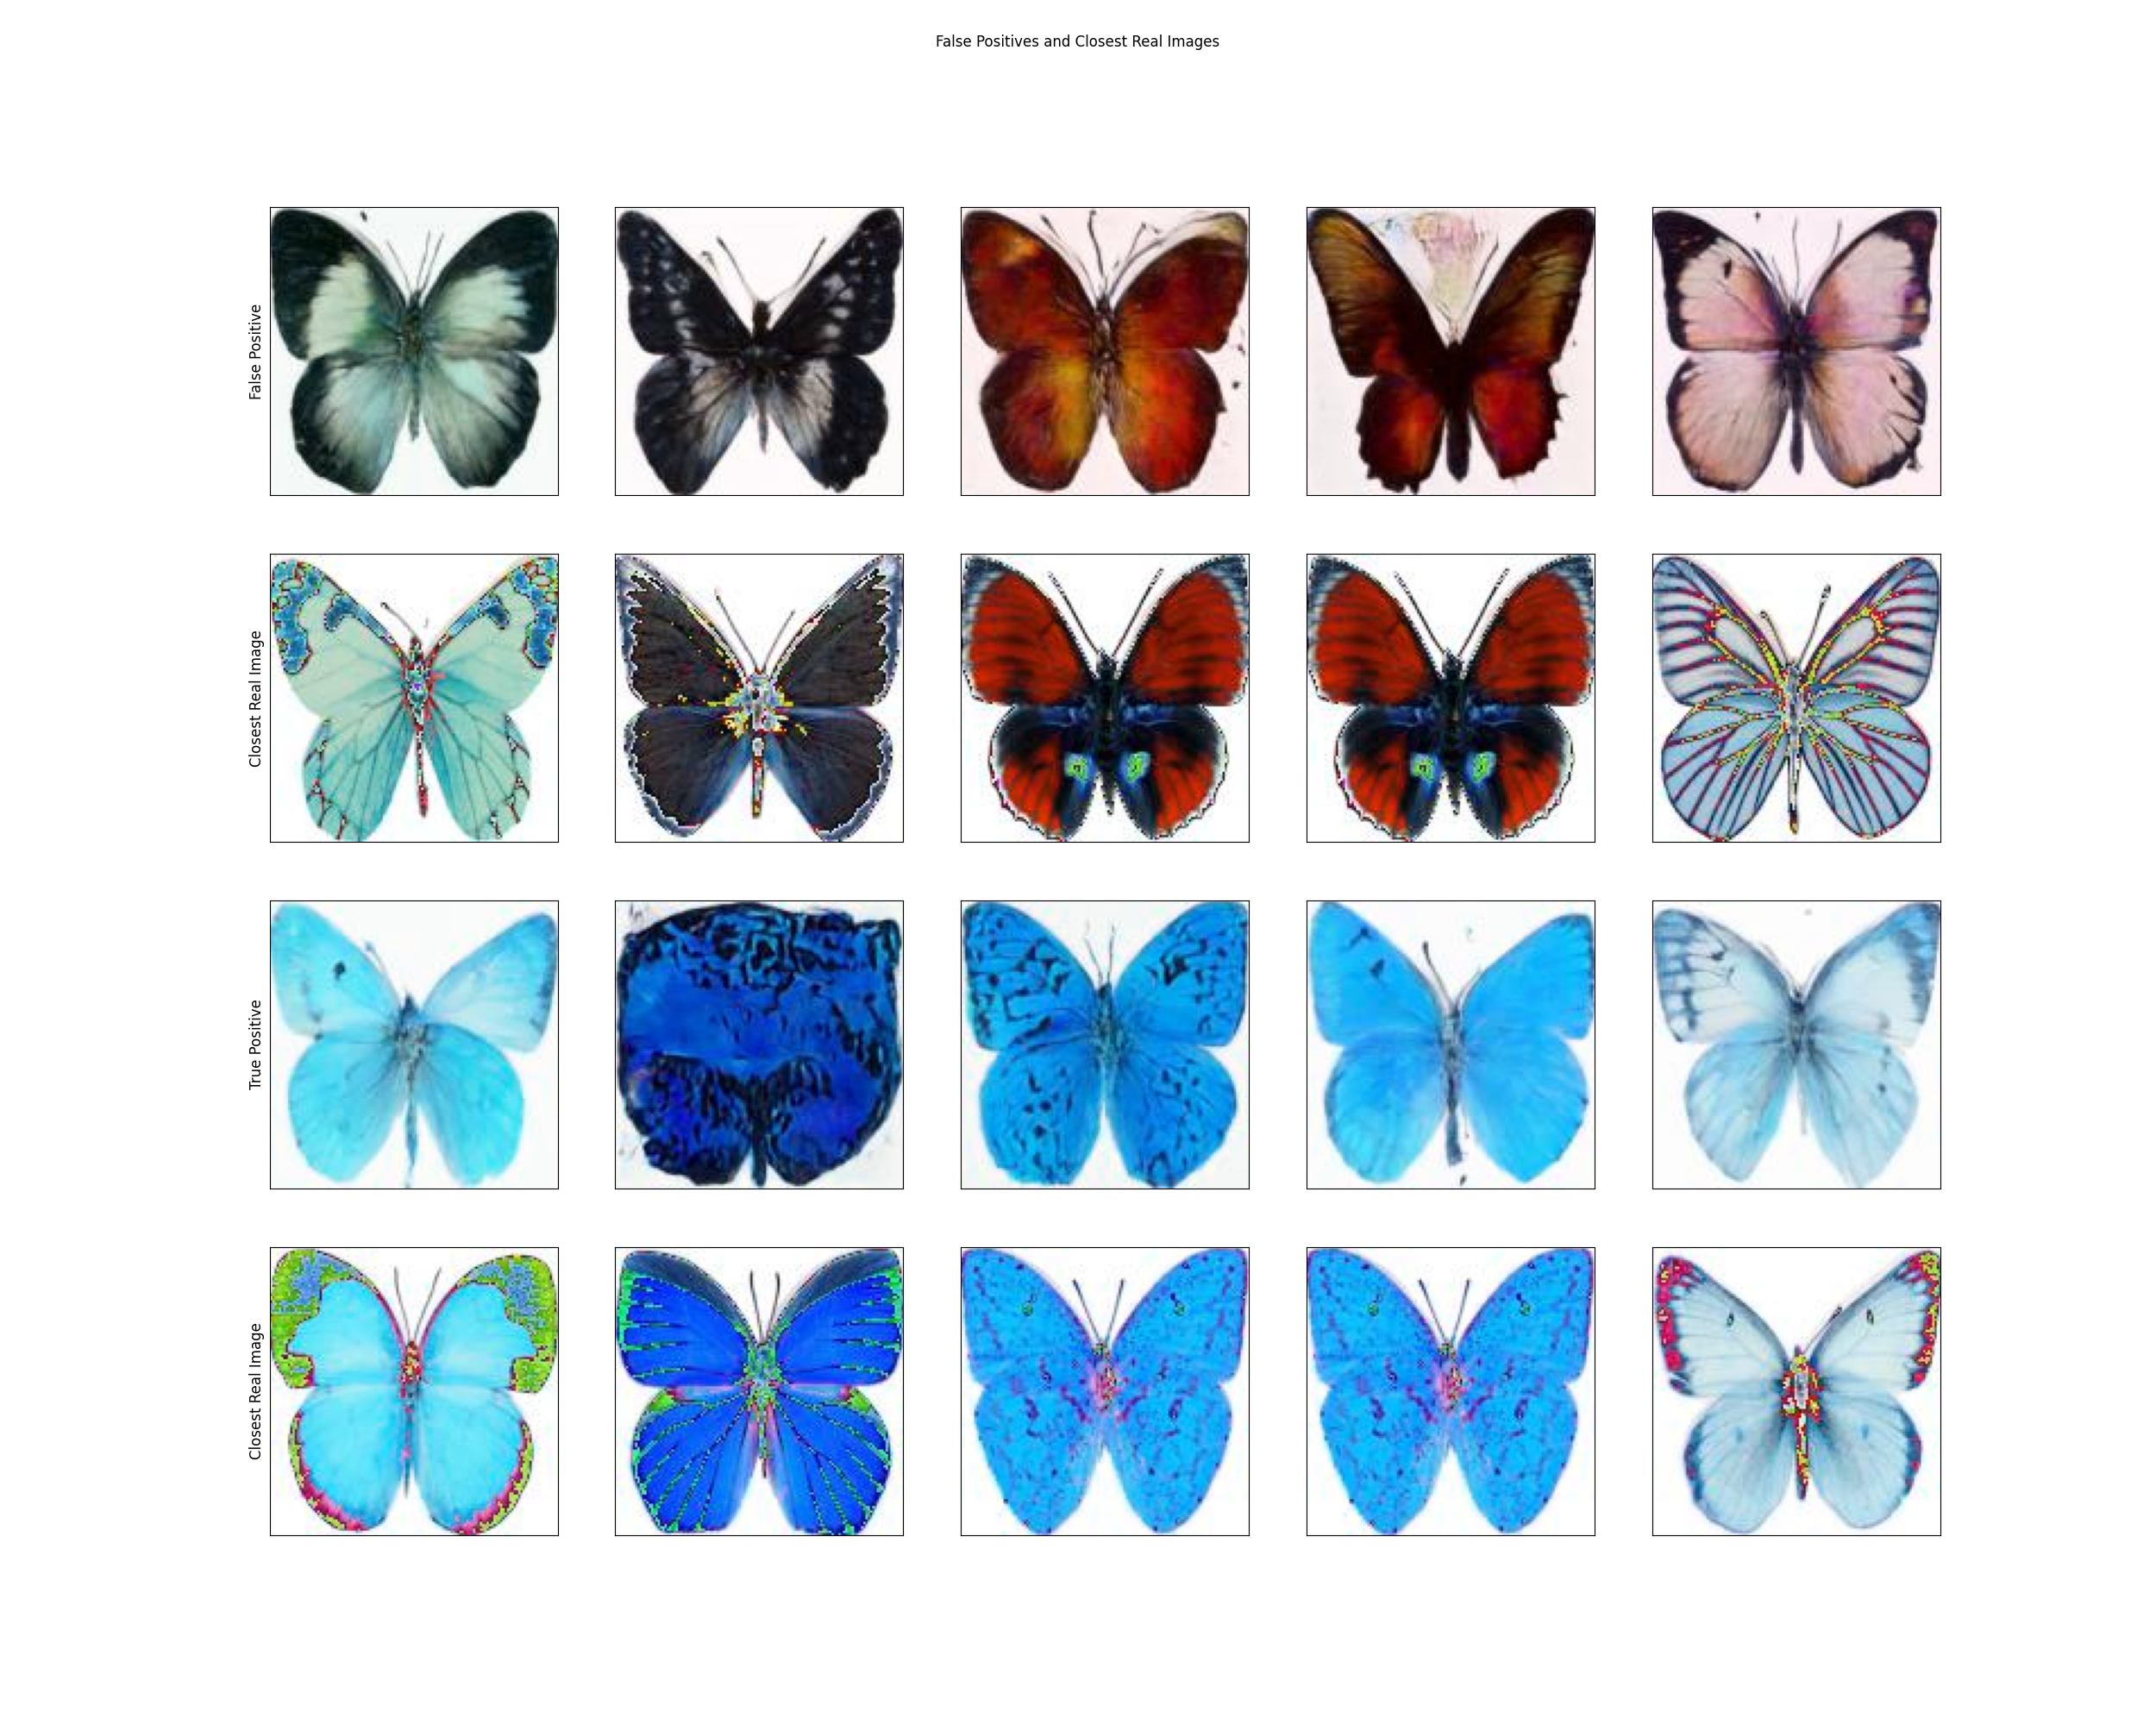
\includegraphics[width=0.45\textwidth]{../images/realworldexperiments/butterflies/examples/fp_hsv_histogram.png}
\end{figure}
\begin{figure}[!ht]
    \centering
    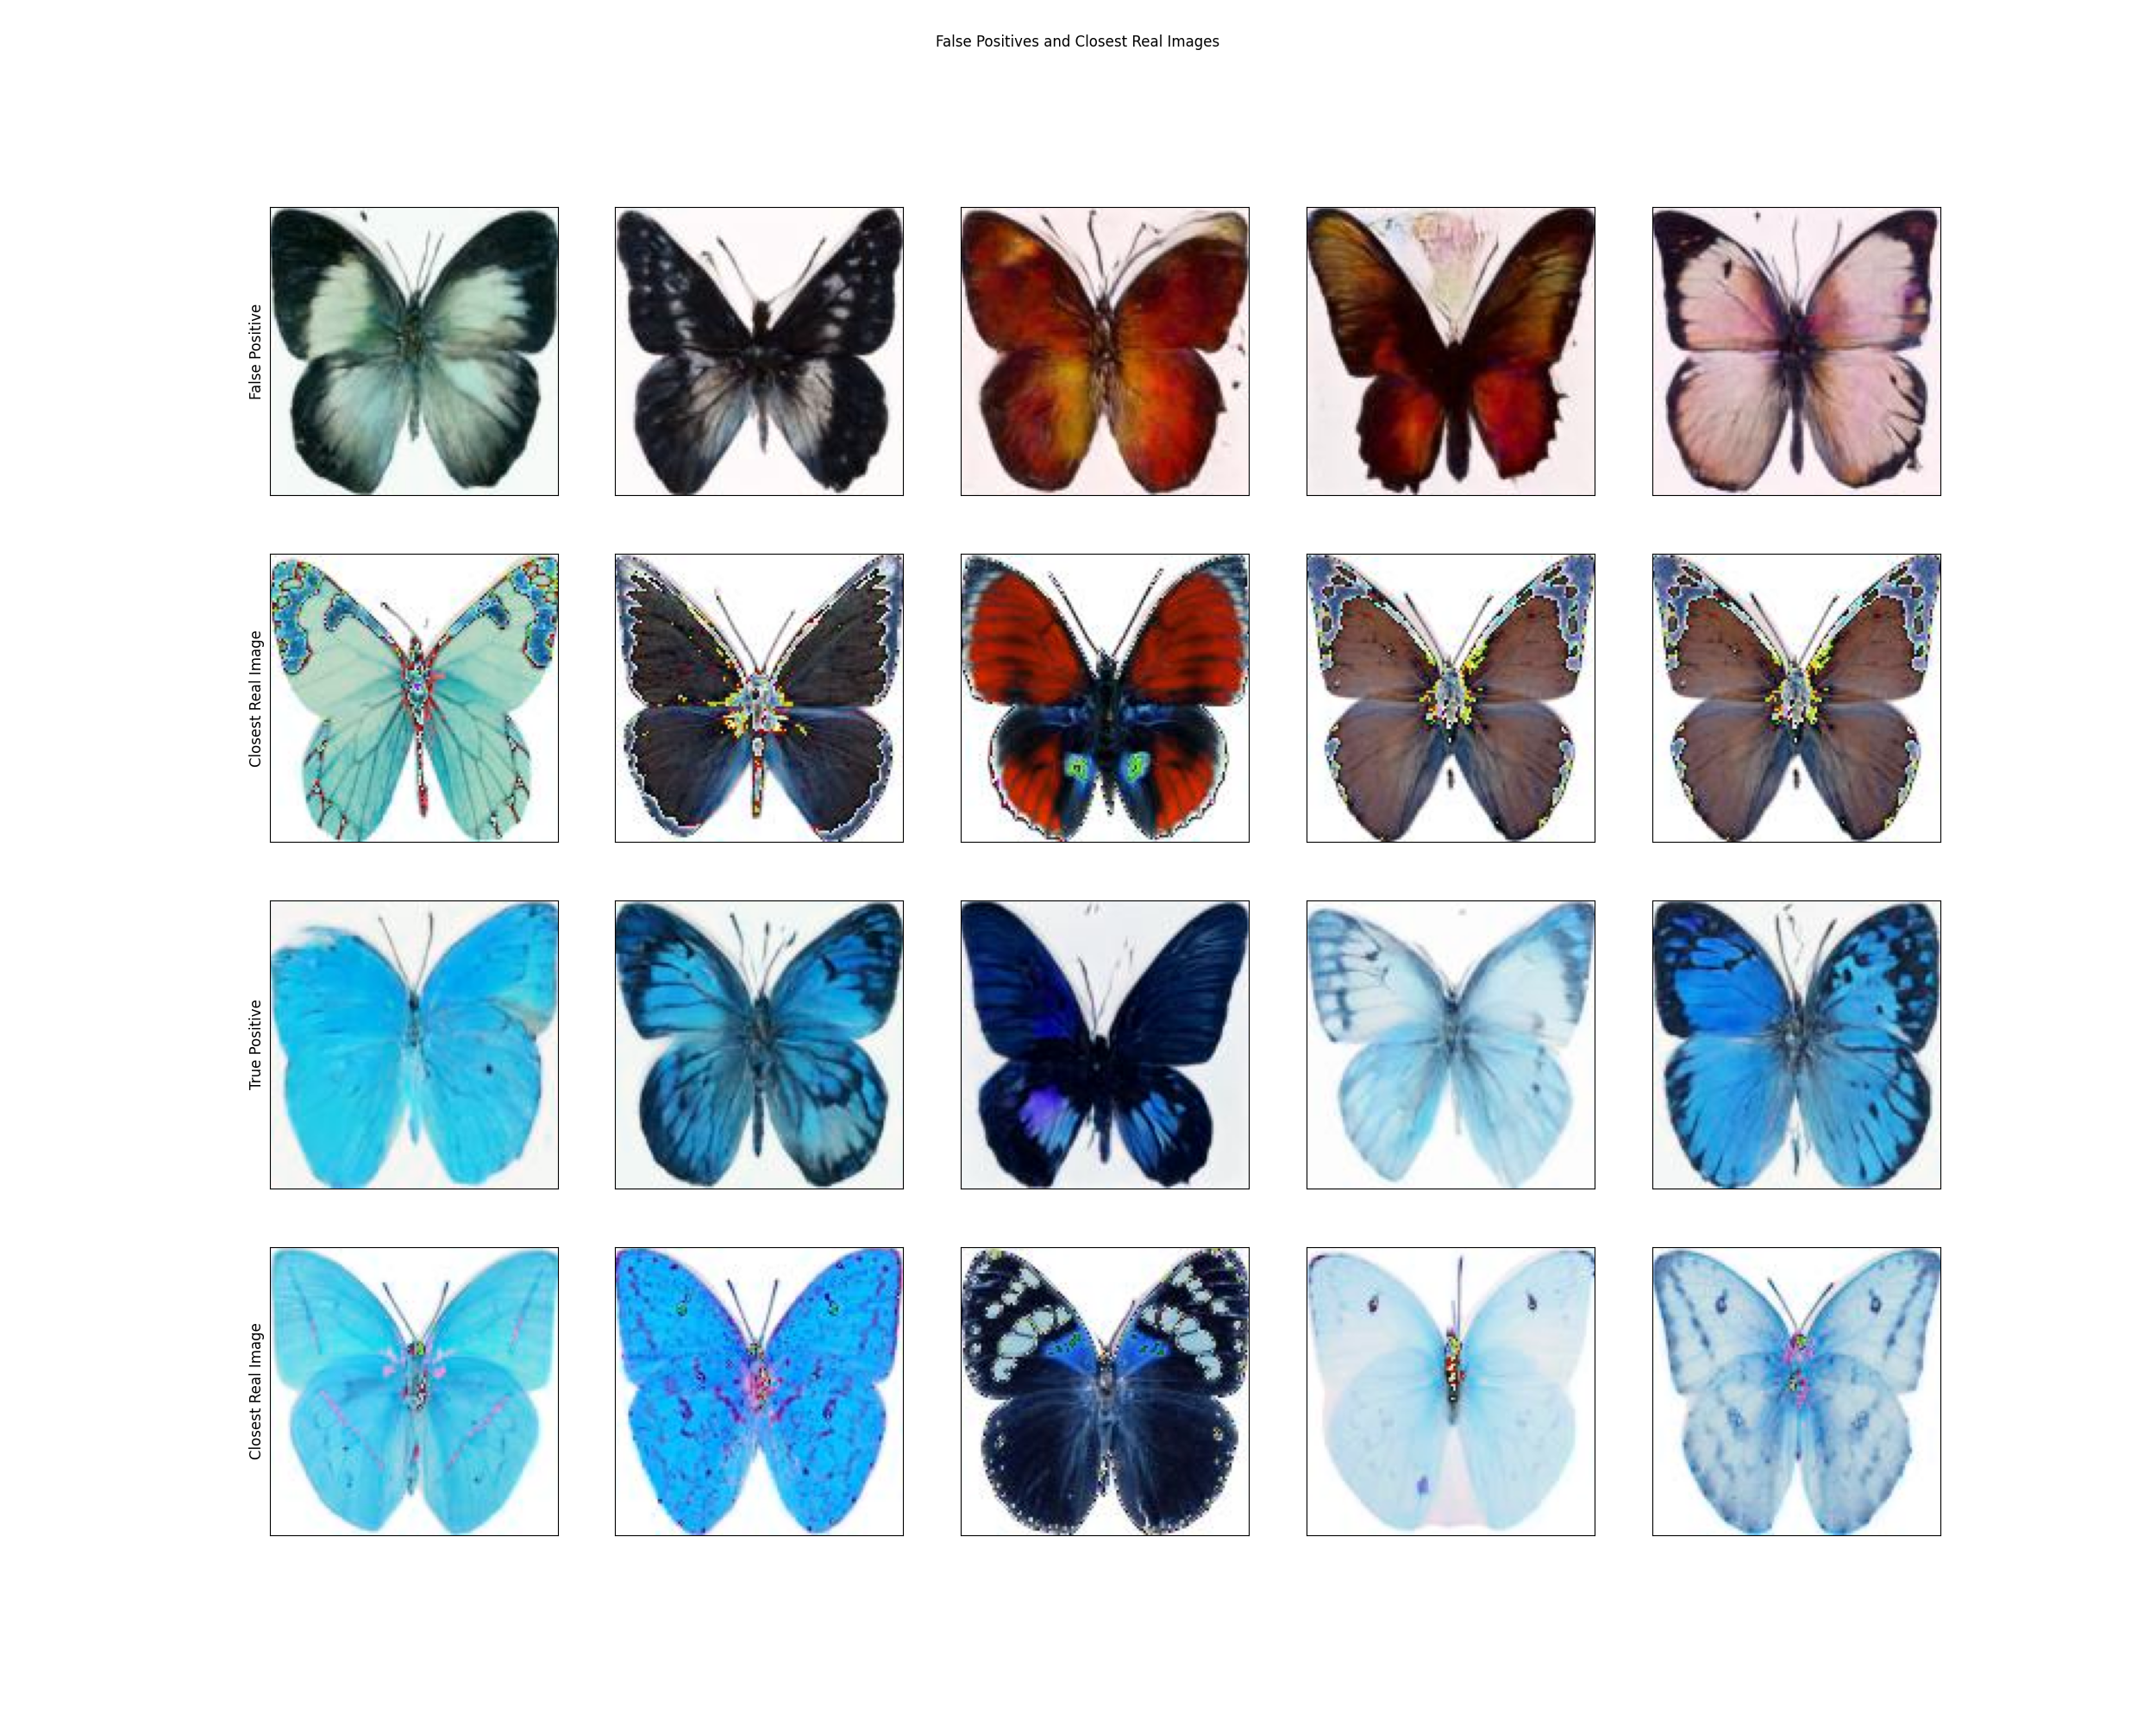
\includegraphics[width=0.45\textwidth]{../images/realworldexperiments/butterflies/examples/fp_hue_histogram.png}
    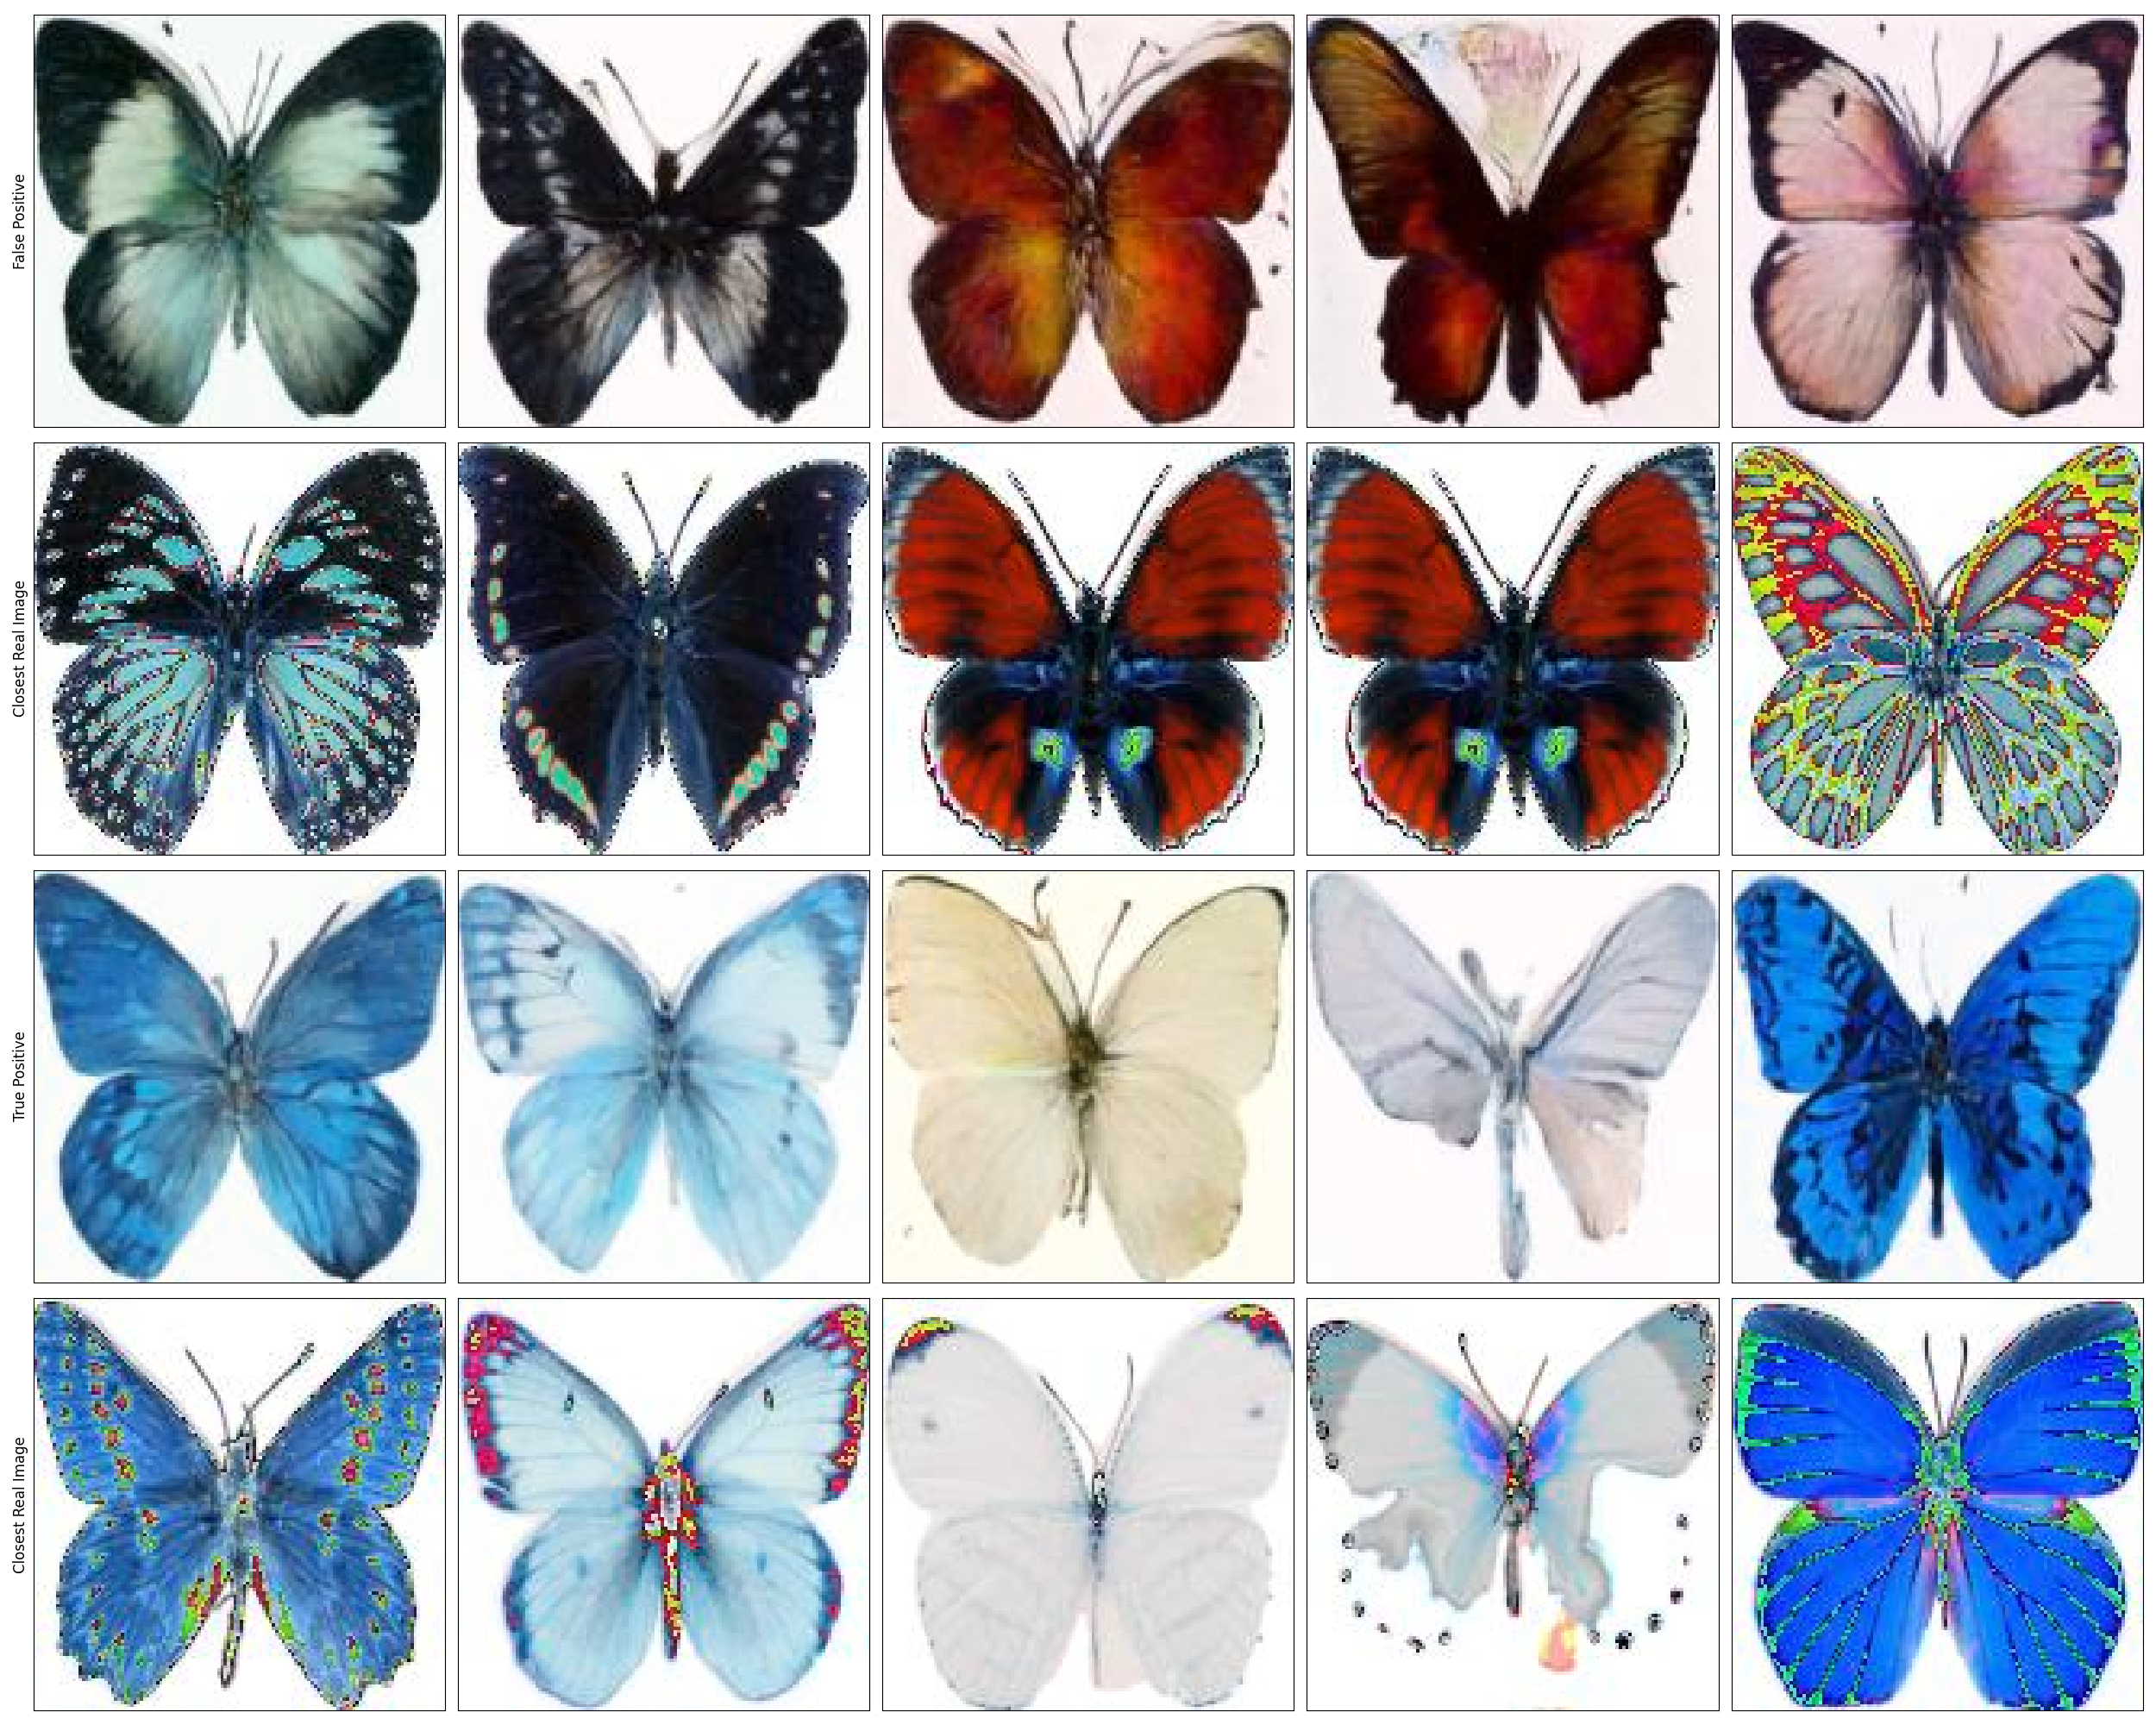
\includegraphics[width=0.45\textwidth]{../images/realworldexperiments/butterflies/examples/fp_rgb_histogram.png}
    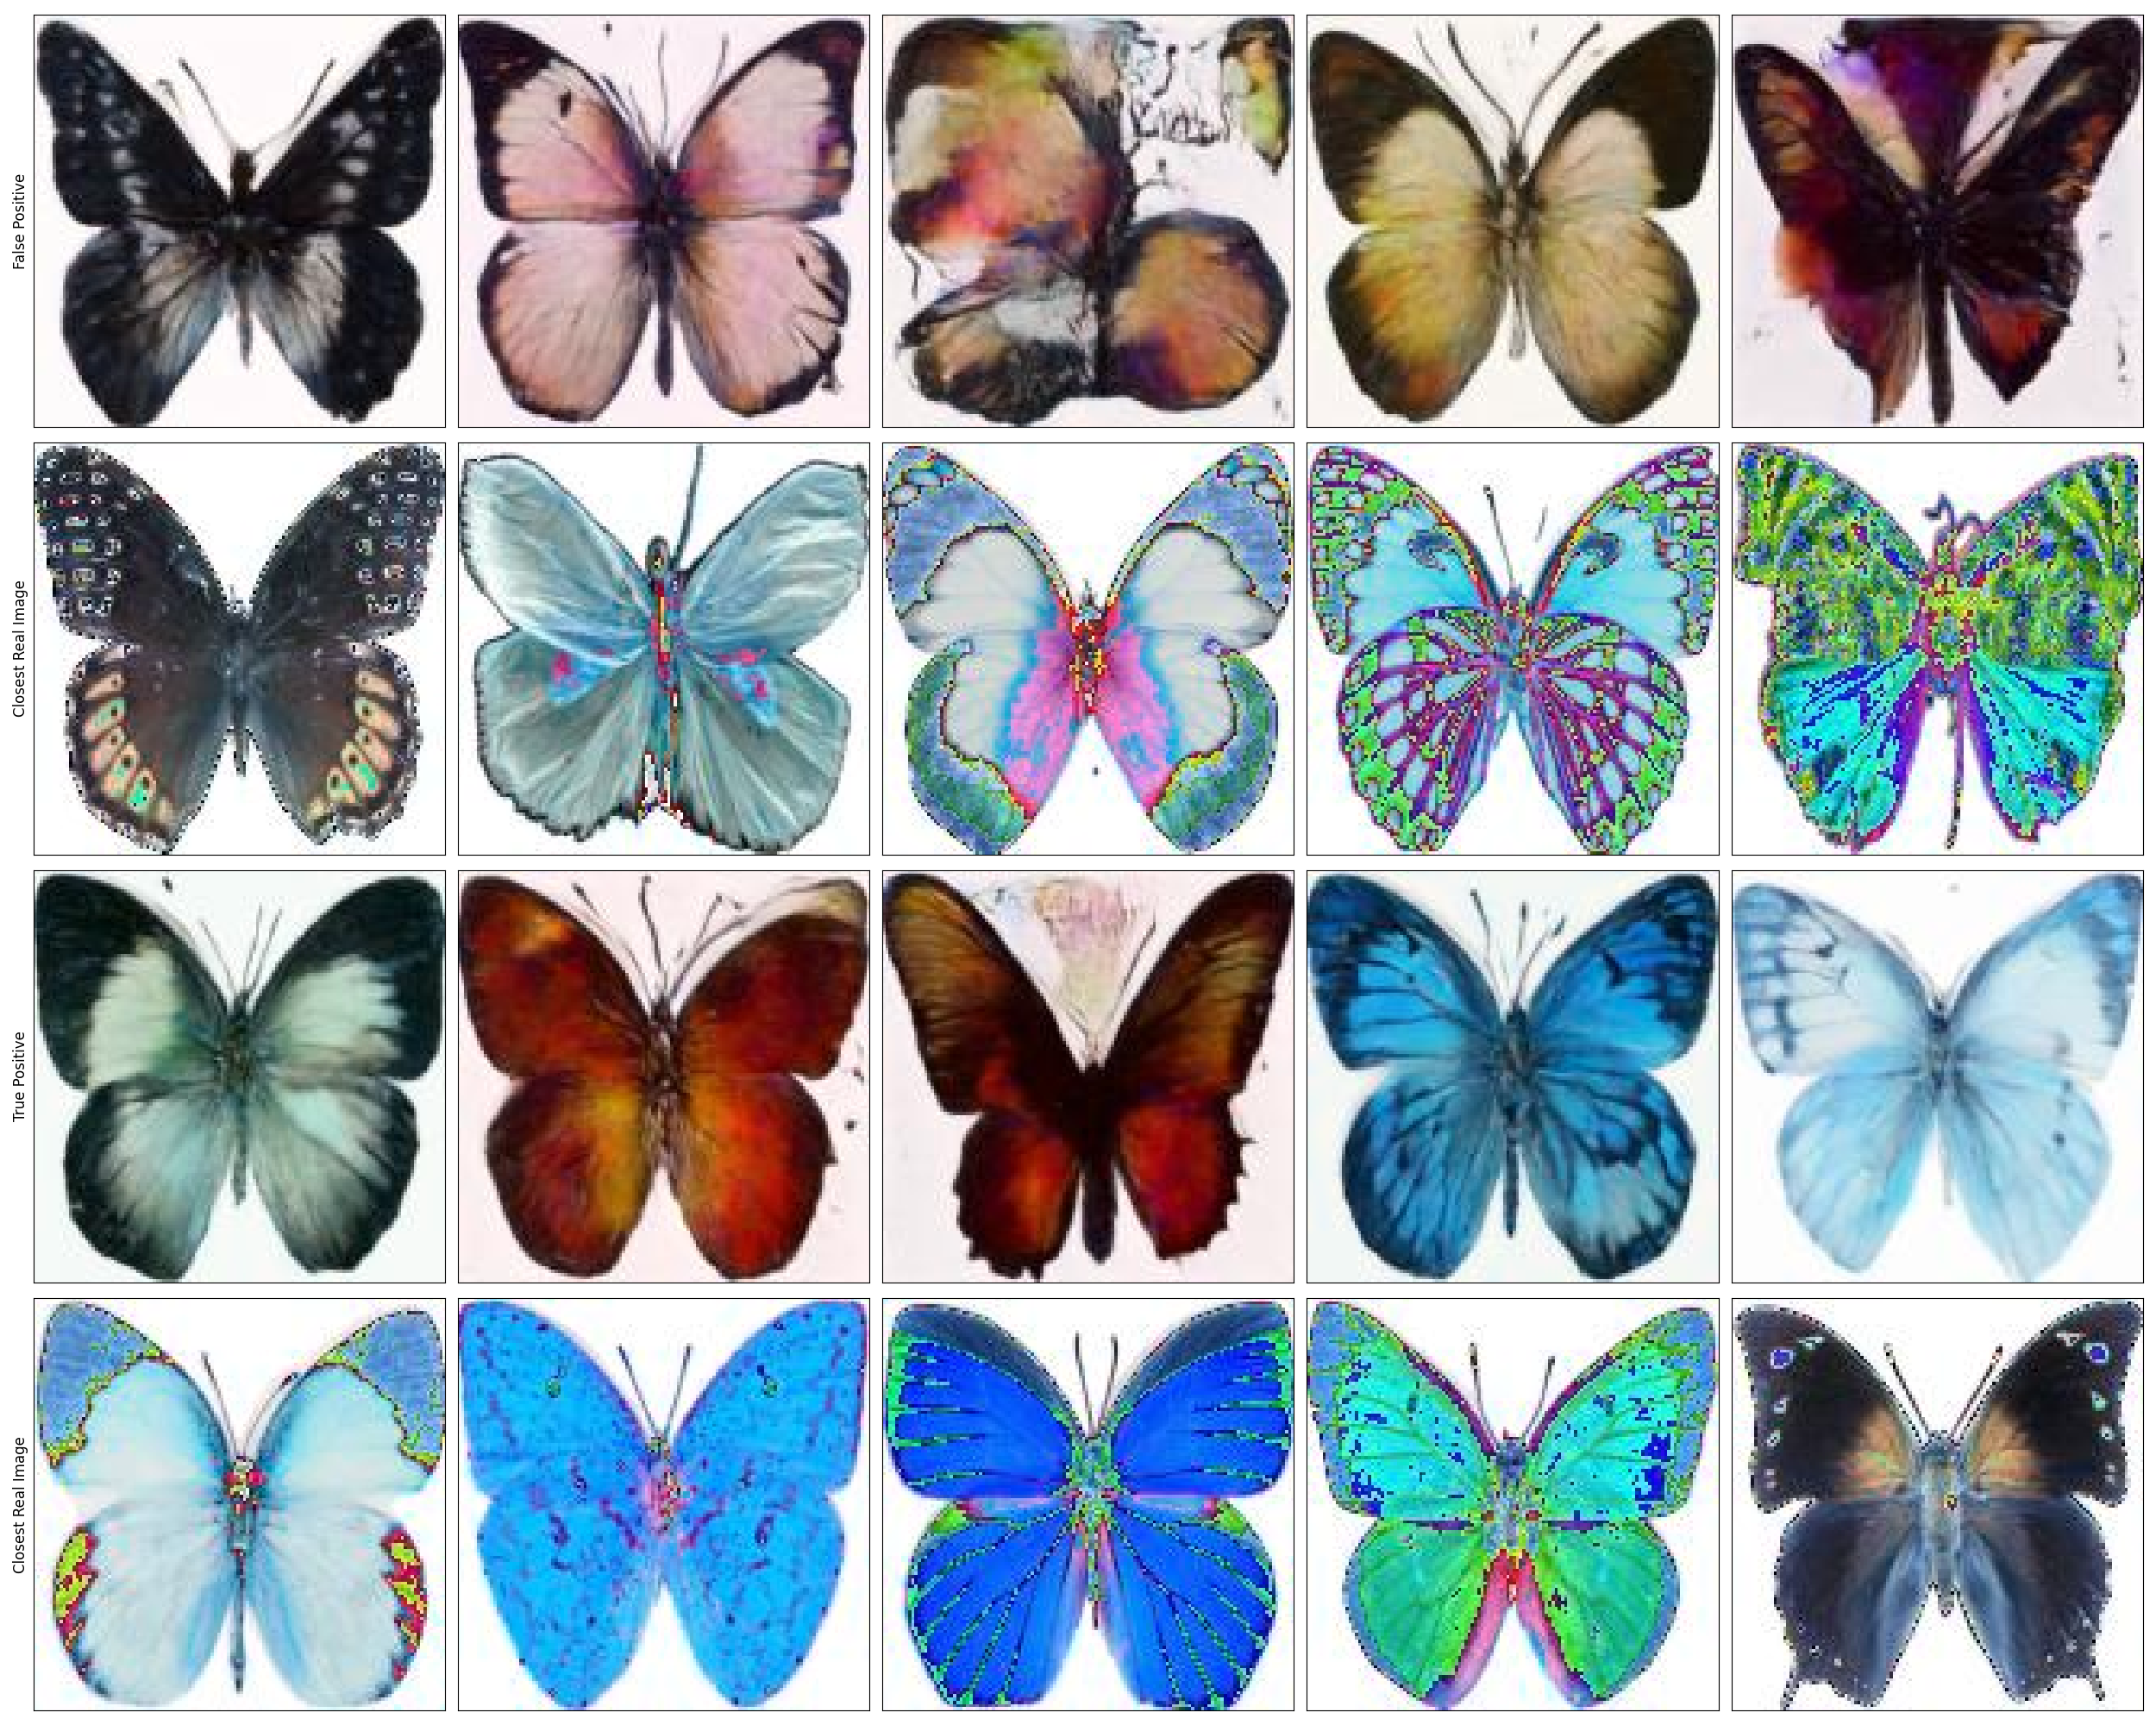
\includegraphics[width=0.45\textwidth]{../images/realworldexperiments/butterflies/examples/fp_saturation_histogram.png}
    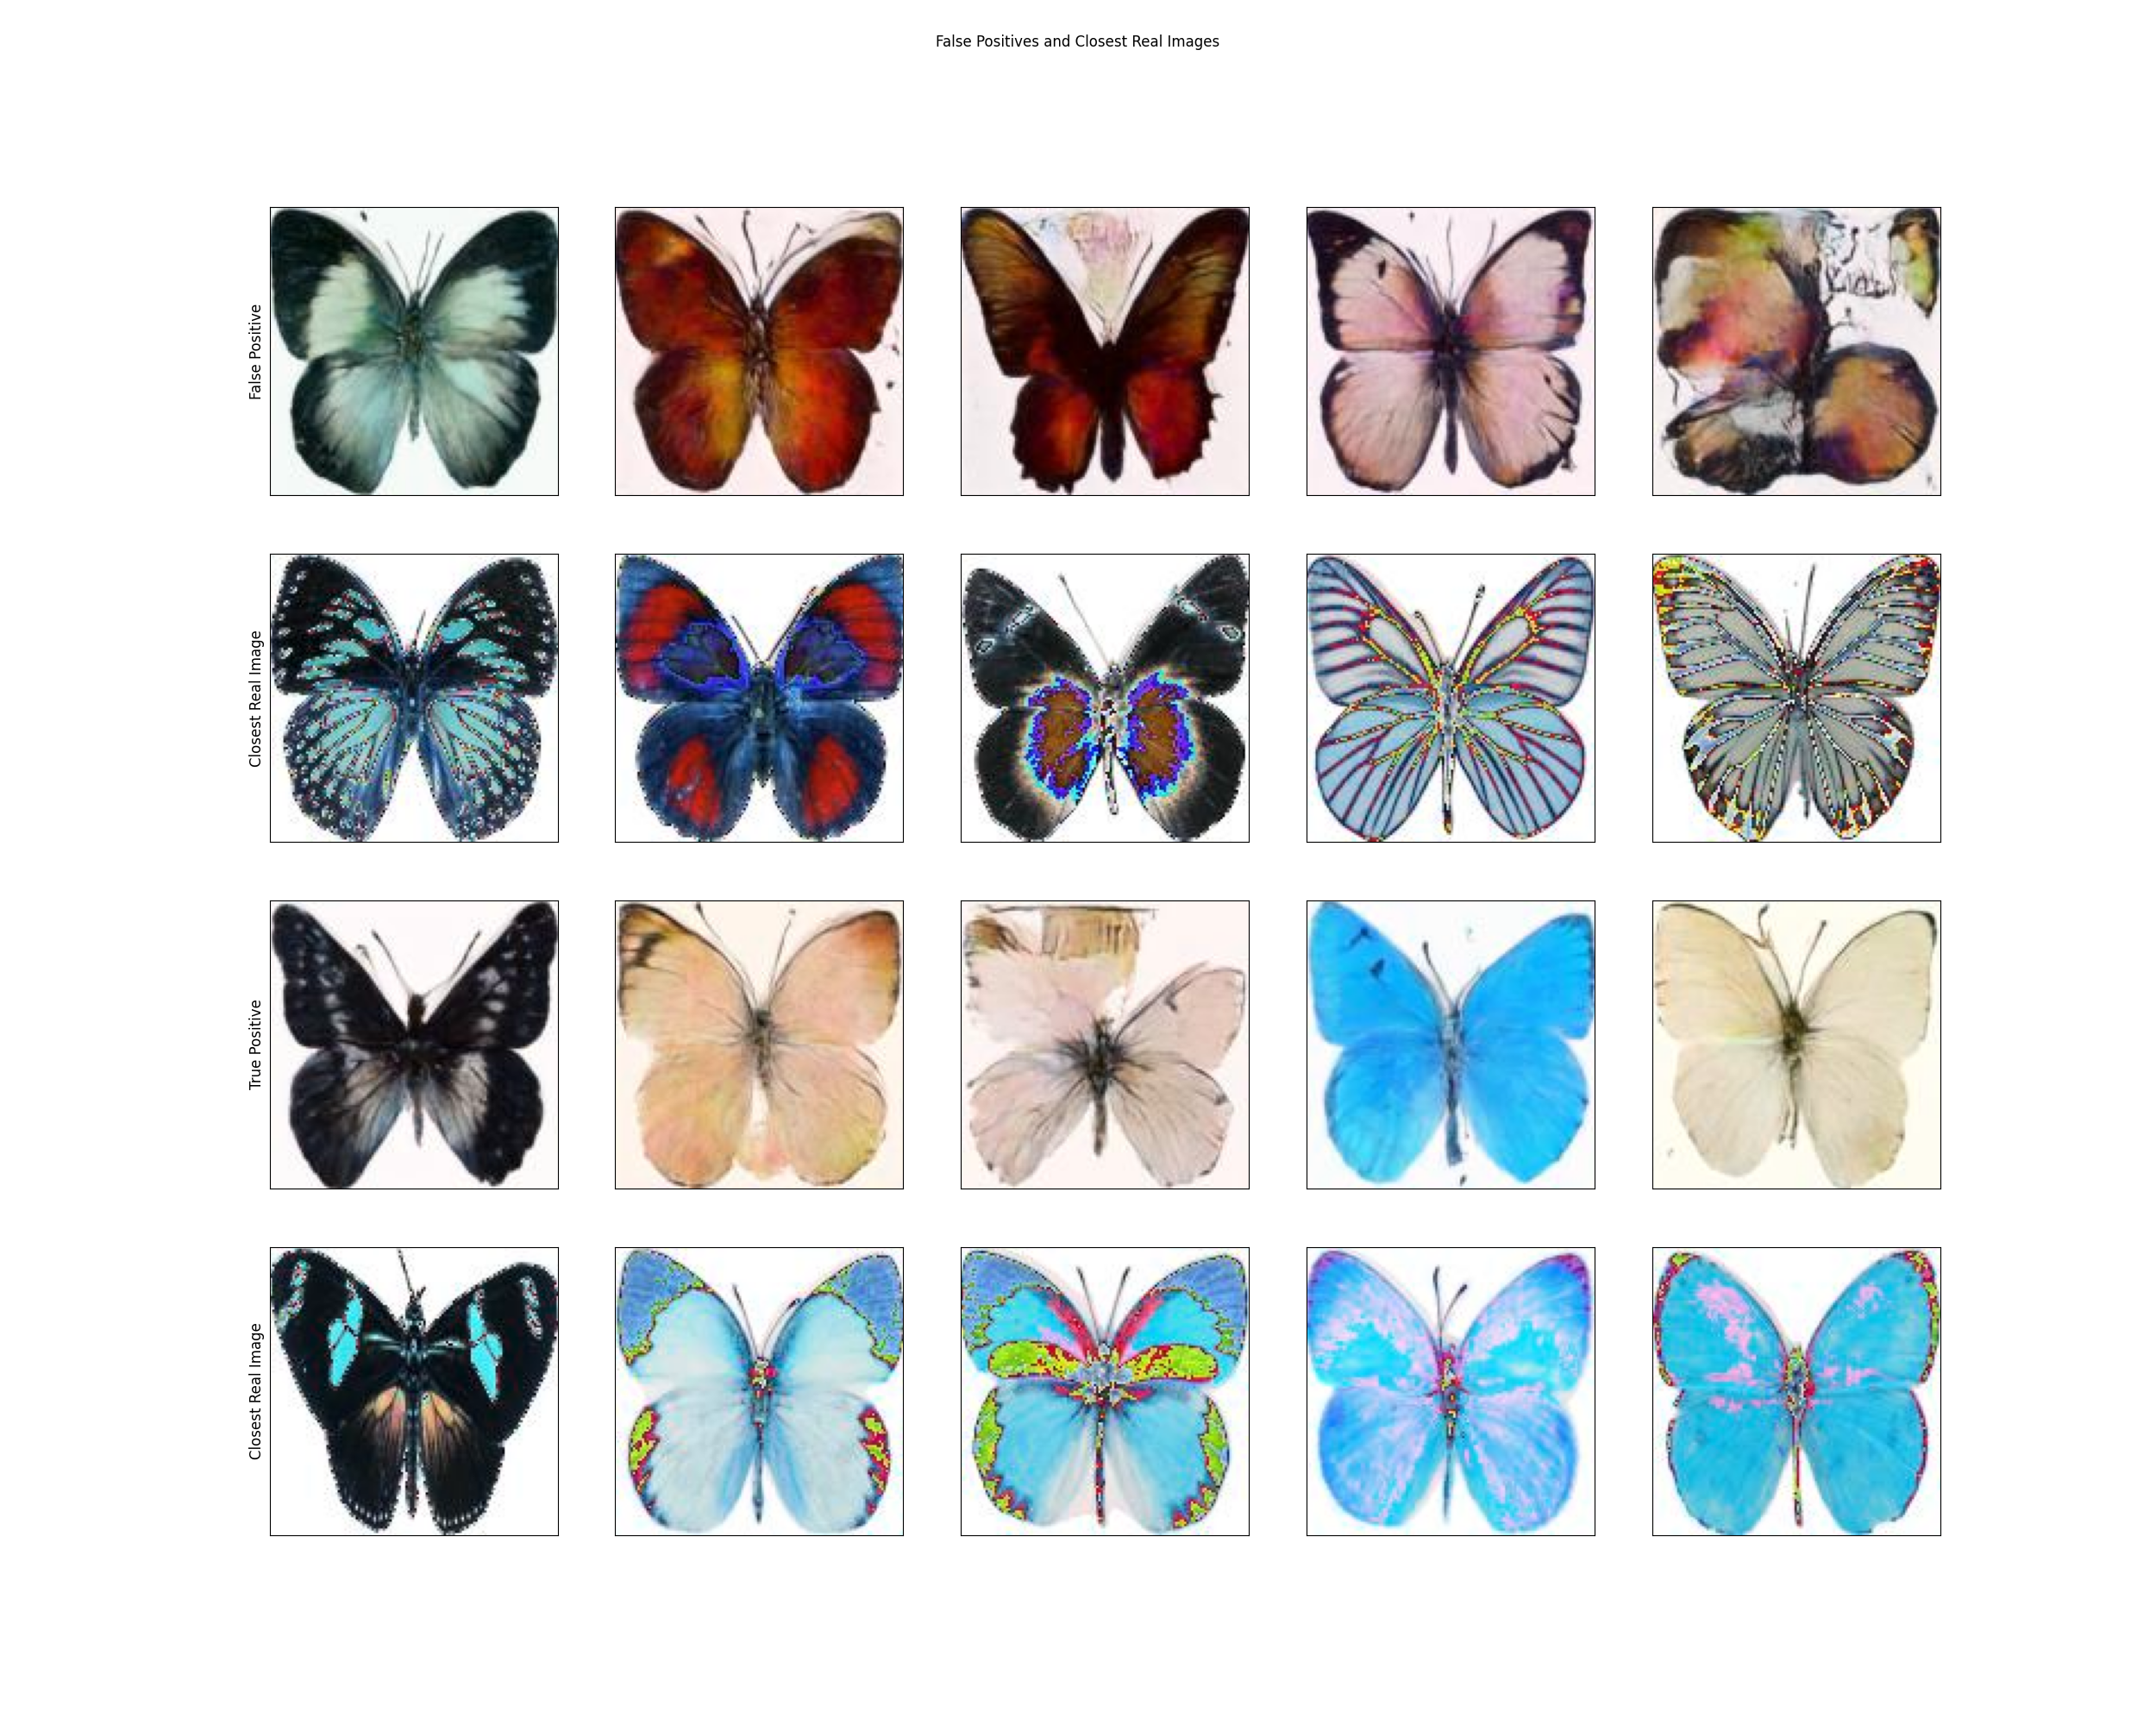
\includegraphics[width=0.45\textwidth]{../images/realworldexperiments/butterflies/examples/fp_value_histogram.png}
    \caption{l'ordine delle immagini da sinistra verso destra e dall'alto in basso è: grayscale, hsv, hue, rgb, saturation, value}
\end{figure}

\subsection{Scarlatti}